\documentclass[a4j]{jarticle}%[a4j]
%\documentclass[10pt,a4j]{jsarticle}%[twocolumn,10pt,a4j]{jsarticle}
%-------Package--------------
%you can add package
\usepackage{float}
\usepackage{amsmath,amssymb, bm}%equation
%\usepackage{wrapfig}
\usepackage[dvipdfmx]{graphicx,hyperref}%pdf%[draft]{graphicx}%
\usepackage{pxjahyper}
\hypersetup{
	colorlinks=false, % リンクに色をつけない設定
	bookmarks=true, % 以下ブックマークに関する設定
	bookmarksnumbered=true,
	pdfborder={0 0 0},
	bookmarkstype=toc
}
\usepackage[dvipdfmx]{color}
\usepackage{multicol}
\usepackage{url}
\usepackage{color}

\renewcommand{\contentsname}{目次}%contents name
\renewcommand{\abstractname}{概要}%abstract name
\renewcommand{\appendixname}{付録}%appendix name
\renewcommand{\refname}{参考文献}%Reference name
%-------margin-------------
\usepackage[top=25truemm,bottom=25truemm,left=25truemm,right=25truemm]{geometry}

%%%   section setup   %%%
\makeatletter

\def\section{\@startsection {section}{1}{\z@}
{\ifnum \c@section = 0
0.0ex plus
\else
-2.0ex plus 
\fi
 -1ex minus -.2ex}
{0.3ex plus .2ex}{\reset@font\fontsize{14pt}{0pt}\gtfamily\sffamily}}%{\normalsize\bf}}%section bf and section margin if you need more margin after section number you change ex parameter
%\def\section{\@startsection {section}{1}{\z@}{-2.0ex plus -1ex minus -.2ex}{0.3ex plus .2ex}{\reset@font\gtfamily\sffamily}}%{\normalsize\bf}}%section bf and section margin if you need more margin after section number you change ex parameter

%%%   PAGE STYLE   %%%
\usepackage{fancyhdr}
\pagestyle{fancy}

% *** ヘッダーのデザイン、やりかけ、名案求む *** %
%\rhead[\leftmark]{odd}
\rhead{}
\lhead[even]{\leftmark}
\cfoot{\thepage}
%\fancyfoot{}
%\fancyfoot[LE,RO]{\thepage}
%\fancyfoot[LO,RE]{\hspace{1cm}}%\thepage}
%\fancyhead[LE,RO]{\leftmark}

%\renewcommand{\headrulewidth}{0.4pt}
%\renewcommand{\footrulewidth}{0.4pt}

%%%   TITLE PAGE   %%%
\def\@cite#1#2{\hbox{\normalsize{%%%\scriptsize{%参考文献の参照
\if@tempswa(#2)
\else(#1)
\fi}}}

\def\@biblabel#1{\hbox{$\cdot$}}%参考文献リストの形式


\renewcommand{\figurename}{Fig. }%fig name
\renewcommand{\tablename}{Tab. }%table name

\renewcommand{\thefigure}{\thesection.\arabic{figure}}
\@addtoreset{figure}{section}%図のタイトル

\renewcommand{\thetable}{\thesection.\arabic{table}}
\@addtoreset{table}{section}%表のタイトル

\renewcommand{\theequation}{\thesection.\arabic{equation}}
\@addtoreset{equation}{section}%数式のタイトル

\def\figref#1{\hbox{Fig. \ref{#1}}}%図の参照
\def\tabref#1{\hbox{Tab. \ref{#1}}}%表の参照
\def\eqref#1{\hbox{Eq. \ref{#1}}}%式の参照


\def\thesis#1{\def\@thesis{#1}}
\def\id#1{\def\@id{#1}}
\def\department#1{\def\@department{#1}}
\def\sensei#1{\def\@sensei{#1}}
 \def\@maketitle{%
 \begin{center}%
 \let\footnote\thanks%
   \hbox{ }
   \vspace{10mm}%
   {\LARGE \@thesis \par}%
   \vspace{50mm}%
   {\Huge \@title \par}%title font large=12pt
   \vspace{50mm}%
   {\LARGE \@department \par}%
   \vspace{1mm}%
   {\LARGE 学籍番号 \@id \par}%
   \vspace{1mm}%
   {\LARGE \@author \par}%
   \vspace{20mm}%
   {\LARGE 指導教員 \@sensei \par}%
 \end{center}%
 \vskip\Cvs%
 }
\makeatother 

%%%%%%%%%%%%%%%%%%%%%%%%
%%%% New Commands %%%%
%%%%%%%%%%%%%%%%%%%%%%%%
% Vector
\def\bvec#1{\hbox{\boldmath $#1$}}%Bold style vector
% degree, arcmin, arcsec
\def\degr{\hbox{$^\circ$}}
\def\arcmin{\hbox{$^\prime$}}
\def\arcsec{\hbox{$^{\prime\prime}$}}
% thermal degree
\def\degc{\hbox{$^\circ$C}}
\def\degf{\hbox{$^\circ$F}}
% greece alphavet
\def\alp{\hbox{$\alpha$}}
\def\bet{\hbox{$\beta$}}
\def\gam{\hbox{$\gamma$}}
\def\x{\hbox{$\times$}}

%-------Thesis Title and Author Name------------
\thesis{2018年度~~修士論文}
\title{非対称SNR~G350.1-0.3におけるイジェクタ噴出速度の測定 \\ Measurement of ejecta velocity in an irregular galactic supernova remnant G350.1-0.3}
\department{理学研究科~物理学専攻}
\id{17LA012Z} 
\author{湯澤~洋治}
\sensei{内山泰伸}

%-------Body------------
\begin{document}

%タイトルの表示
\maketitle
\newpage

%-------はじめに------------
%概要の記述(研究の意義、歴史史的に、かつ物理的にどういう意義があるのか)
\section{概要}
\begin{abstract}

\end{abstract}

\newpage
% 目次の表示
\tableofcontents
\newpage

%%%%%%%%%%%%%%%%%%%%%%%%%%%%

%%%%%%%%%%%%%%%%%%%%%%%%%%%%
%------- Aboout SNe ------------
\section{超新星爆発}

%------- Aboout Atomic fusion process ------------
\subsection{恒星内部の核融合反応}



%------- Aboout SN process ------------
\subsection{超新星}



%------- Aboout SN process ------------
\subsection{非球対称な超新星爆発}



%%%%%%%%%%%%%%%%%%%%%%%%%%%%
%------- Aboout SNR ------------
\section{超新星残骸}

%------- Aboout SNR ------------
\subsection{導入}



%------- Aboout optically thin plasma ------------
\subsection{光学的に薄いプラズマ}

%------- Aboout SNR physical process ------------
\subsection{超新星残骸における物理現象}

\newpage
%%%%%%%%%%%%%%%%%%%%%%%%%%%%
%------- Aboout SNR  ------------
\section{超新星残骸~G350.1-0.3}
\subsection{概要}
 G350.1-0.3は(RA,Dec)=(17h21m05s,-37$^\circ$.27)に位置する年齢1000--2000歳の若い超新星残骸である。これまで赤外、電波及びX線で観測されており、それぞれの波長でその特異な形状が異なることが確認されている。日本のX線観測衛星すざくによる観測\cite{Yasumi2014}では、鉄より大きな質量の$\rm{Ni}$が検出されており、非対称な爆発がスペクトル解析から示唆されている。
また、本天体はFig\ref{fig:g350_cxc}のように極端に非対称な形状をとっていることから、超新星爆発における非対称性を噴出物の分布を引き起こすメカニズムに迫るための重要な天体の1つだと考えられる。

\begin{figure}[H]
  \begin{center}
  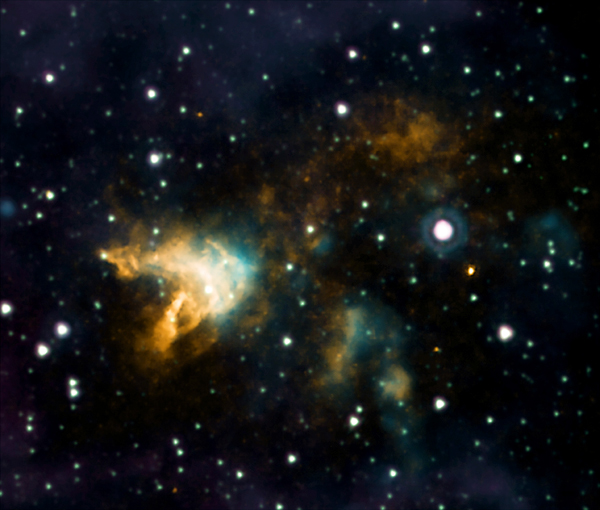
\includegraphics[scale=0.4]{./g350_hand.jpg}
  \caption{超新星残骸G350.1-0.3のイメージ \protect\newline X-ray (Gold) Infrared 24 micron (Cyan) Infrared 8 micron (Purple) Infrared 3.6 micron (Green)}
  \label{fig:g350_cxc}
  \end{center}
  \end{figure}


%  \subsection{\sf{\gt{先行研究}}}
%%%%%%%%%%%%%%%%%%%%%%%%%%%%
%-------  Chandra  ------------
\section{Chandra~X線観測衛星}
\subsection{概要}

\subsection{ACIS}

\subsection{HRMA}

\subsection{エネルギー分解能}

\subsection{エネルギー分解能のキャリブレーション不定性}
%%%%%%%%%%%%%%%%%%%%%%%%%%%%
%------- Chandra analysis ------------
\section{Chandra によるX線解析}
 今回、Chandraによって、table.\ref{tab:1}に示すデータとNASAが提供するCIAO(version~4.9)、Xspec(version~12.9)を使用し、解析を行った。
\begin{table}[H]
  \begin{center}
    \begin{tabular}{cccc}
  \hline
  観測日時       & Observation ID & 観測機器   & 観測時間     \\ \hline
  2009年5月21日 & 10102          & ACIS-S & 82.97 ks \\ \hline
    \end{tabular}
  \end{center}
  \label{tab:1}
  \caption{本研究に用いた観測データ}
\end{table}

\subsection{イメージ解析}
ドップラーシフトの解析を行う領域を決定するために、\textrm{Si,S} の輝線に対して、平均でどれくらいのエネルギーの光子が到来しているのかを示す\textrm{Mean Photon Energy Map(MPE map)}を作成した。
MPE~mapを作成する際は検出器の各ピクセルに以下のような計算を行い、光子の平均エネルギーを求めた。\\
\begin{align}
  E_{mean} = \frac{\sum_{i} E_{i} I_{i}}{\sum_{i} I_{i}} \label{doppler-equation}
\end{align}
\textrm{Si,S}の輝線に対して作成したMPE mapを以下のFig.\ref{fig:mpe_map}に示す。

%%%------region figure-----------%%%%%
\begin{figure}[H]
  \begin{center}
  \begin{tabular}{cc}
  
  \begin{minipage}{0.5\hsize}
  \begin{center}
  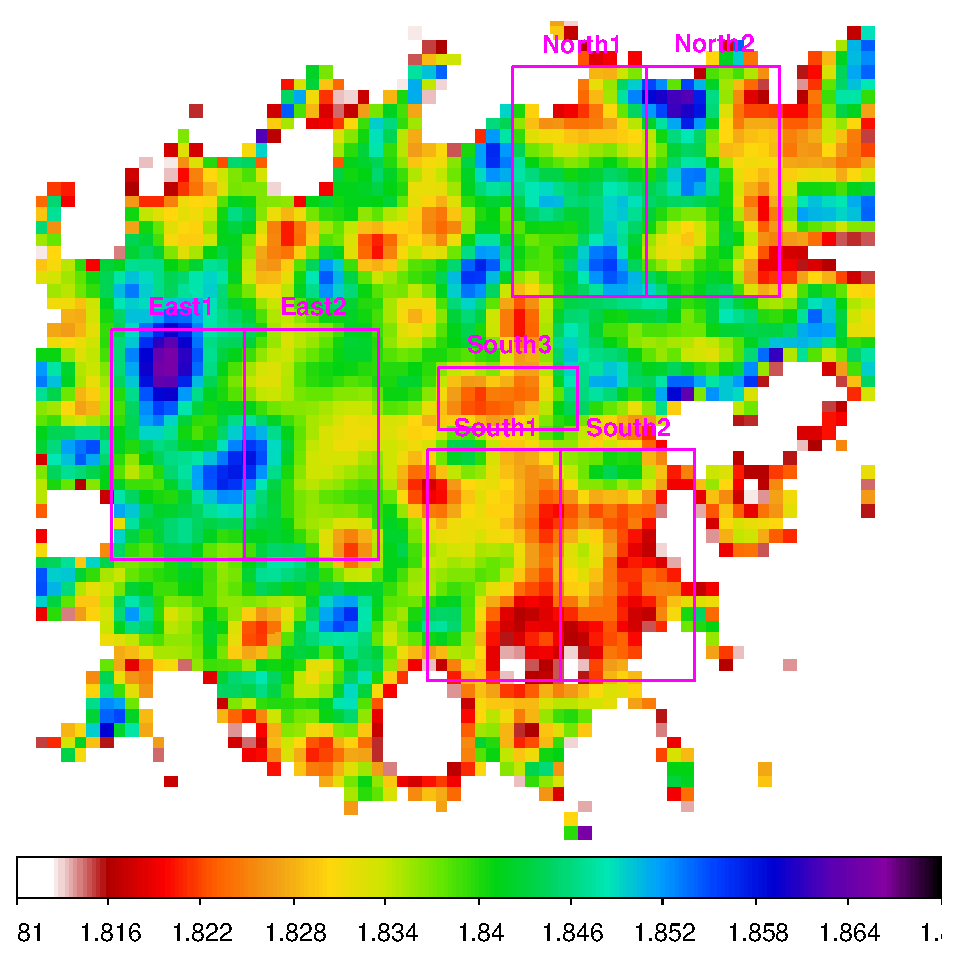
\includegraphics[scale=0.50]{./Si_mean.eps}
  \end{center}
  \end{minipage}
  
  \begin{minipage}{0.5\hsize}
  \begin{center}
  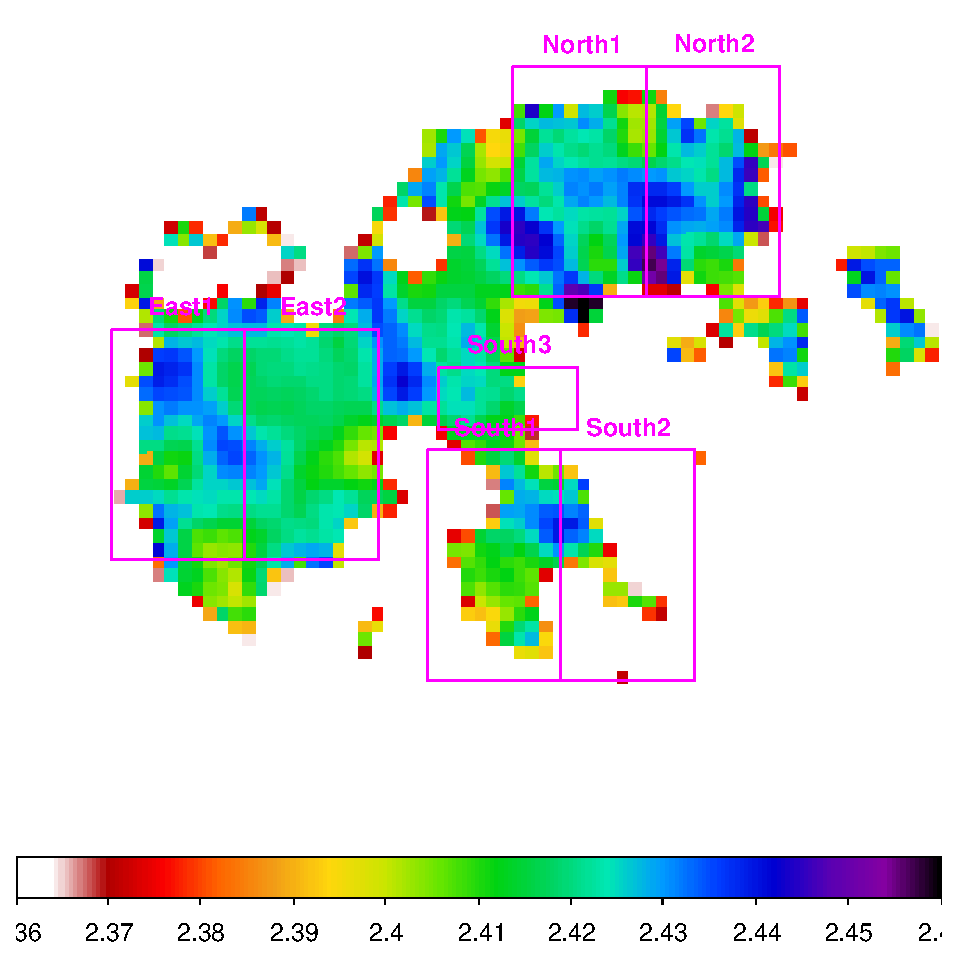
\includegraphics[scale=0.50]{./S_mean.eps}
  \end{center}
  \end{minipage}
  \end{tabular}
  \caption{左図:SiのMean photon energy map(1.6-2.1 keVを35bands $\sim 15 \textrm{keV/band}$に分けて作成した)、右図:SのMean photon energy map(2.2-2.7 keVを34bands $\sim 15 \textrm{keV/band}$に分けて作成した)、どちらも$1\textrm{pixel} \sim 4\textrm{arcsec}$、かつ、$\sigma \sim 12\textrm{arcsec}$でスムージングをかけてある。}
  \label{fig:mpe_map}
  \end{center}
\end{figure}

さらに、輝線の幅の広がりをイメージとして表すためにSiとSのMean photon energy standard  deviation mapをそれぞれ1.6-2.1 keV を 35bands ∼ 15keV/band に分けて作成したものが以下のFig.\ref{fig:std_map}である。Fig.\ref{fig:std_map}$(=S)$は式\ref{std-equation}をもとに作成した。
\begin{align}
  S = \sqrt{\frac{\sum_{i} n_{i}(E_{i}-\bar{E})^2}{\sum_{i} }} = \sqrt{\frac{\sum_{i} n_{i} E^{2}_{i}}{\sum_{i} n_{i}}-(\bar{E})^2} \label{std-equation}
\end{align}

  %%%------region figure-----------%%%%%
\begin{figure}[H]
  \begin{center}
  \begin{tabular}{cc}
  
  \begin{minipage}{0.5\hsize}
  \begin{center}
  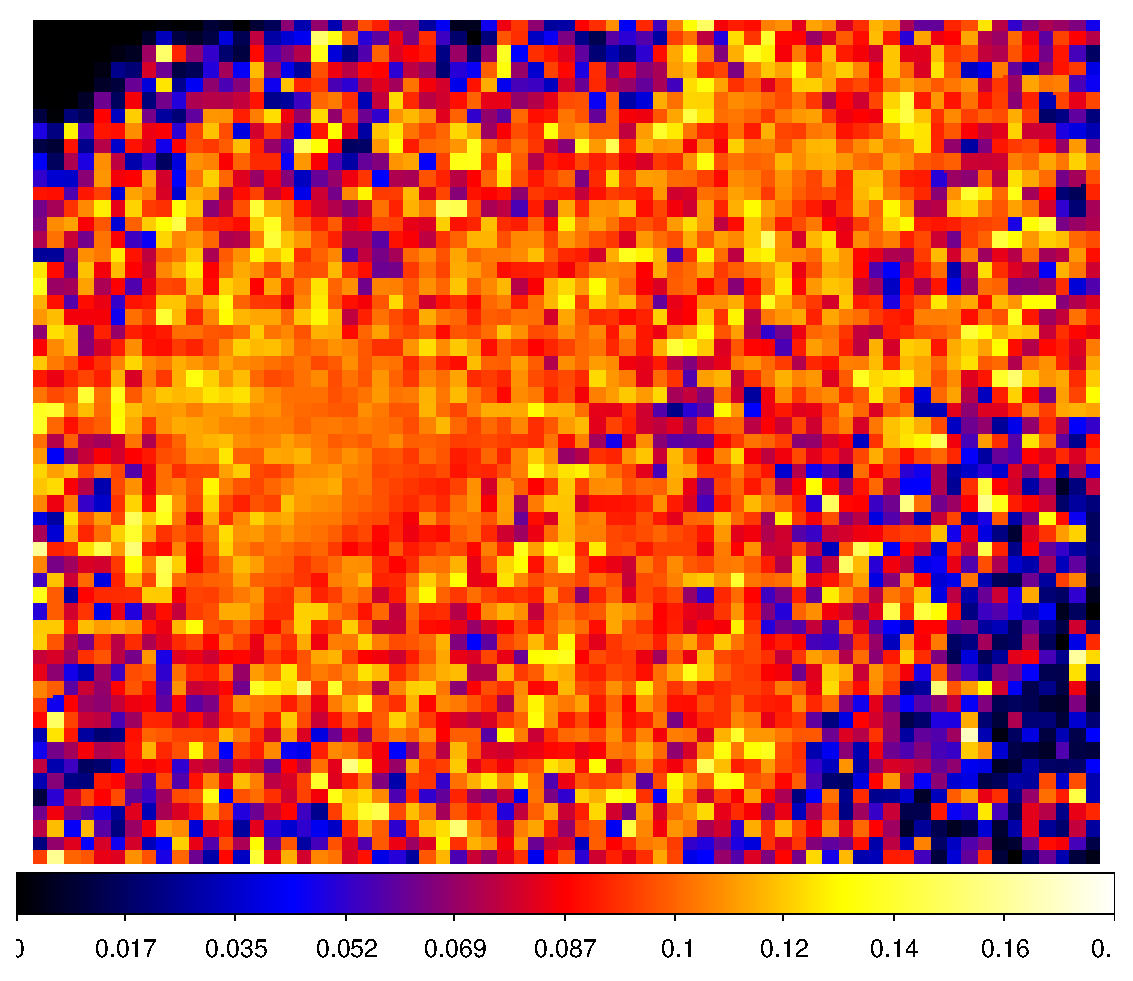
\includegraphics[scale=0.45]{./Si_mean_std.eps}
  \end{center}
  \end{minipage}
  
  \begin{minipage}{0.5\hsize}
  \begin{center}
  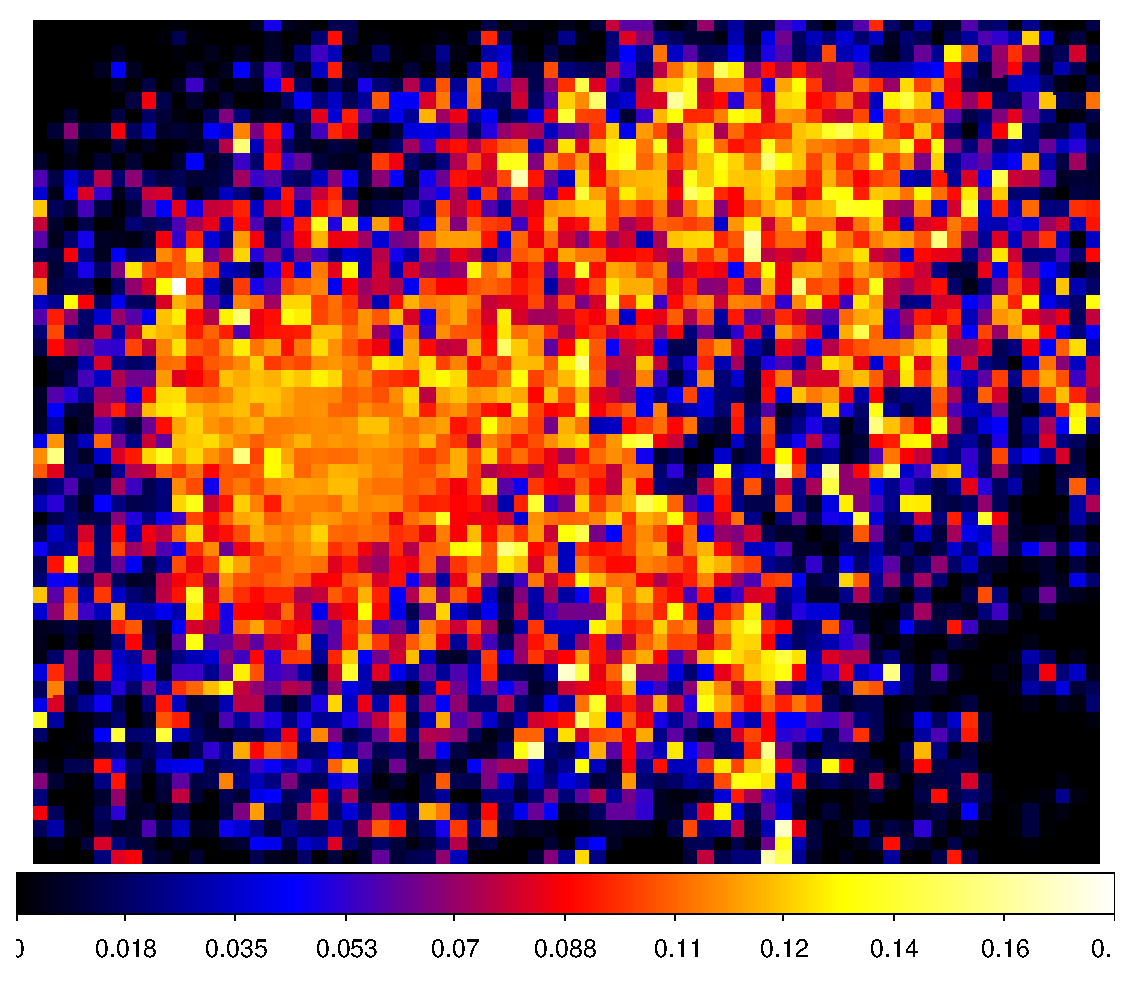
\includegraphics[scale=0.45]{./S_mean_std.eps}
  \end{center}
  \end{minipage}
  \end{tabular}
  \caption{左図:SiのMean photon energy standard deviation map(1.6-2.1 keVを35bands $\sim 15 \textrm{keV/band}$に分けて作成した)、右図:SのMean photon energy standard deviation map(2.2-2.7 keVを34bands $\sim 15 \textrm{keV/band}$に分けて作成した)、どちらも$1\textrm{pixel} \sim 4\textrm{arcsec}$、かつ、$\sigma \sim 8\textrm{arcsec}$でスムージングをかけてある。}
  \label{fig:std_map}
  \end{center}
\end{figure}
  Fig.\ref{fig:mpe_map}から、このSNRでは、南側が青方偏移、北側が赤方偏移の傾向があることがわかる。よって、Fig.\ref{fig:mpe_map}に示すように東、南、北側をそれぞれ、East1,East2,South1,South2,North1,North2,North3に領域を分割した。
本研究では、これらの領域のスペクトル解析を行うことでイジェクタの視線方向の移動速度の計測を行う。

\subsection{スペクトル解析}
SNRのそれぞれの領域のスペクトルをFig.\ref{fig:spec_reg}に示す。Fig.\ref{fig:spec_reg}からも\textrm{Si,S}が偏移していることがわかる。
%%%------region figure-----------%%%%%
\begin{figure}[H]
\begin{center}
\begin{tabular}{cc}

\begin{minipage}{0.5\hsize}
\begin{center}
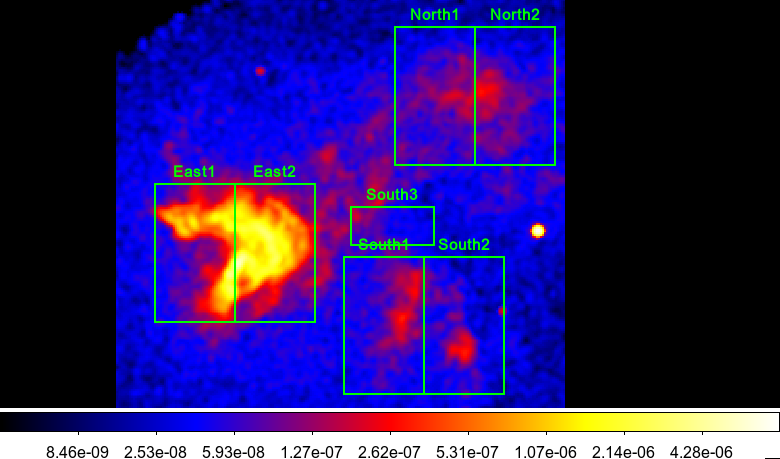
\includegraphics[scale=0.35]{./paper_region.png}
\end{center}
\end{minipage}

\begin{minipage}{0.5\hsize}
\begin{center}
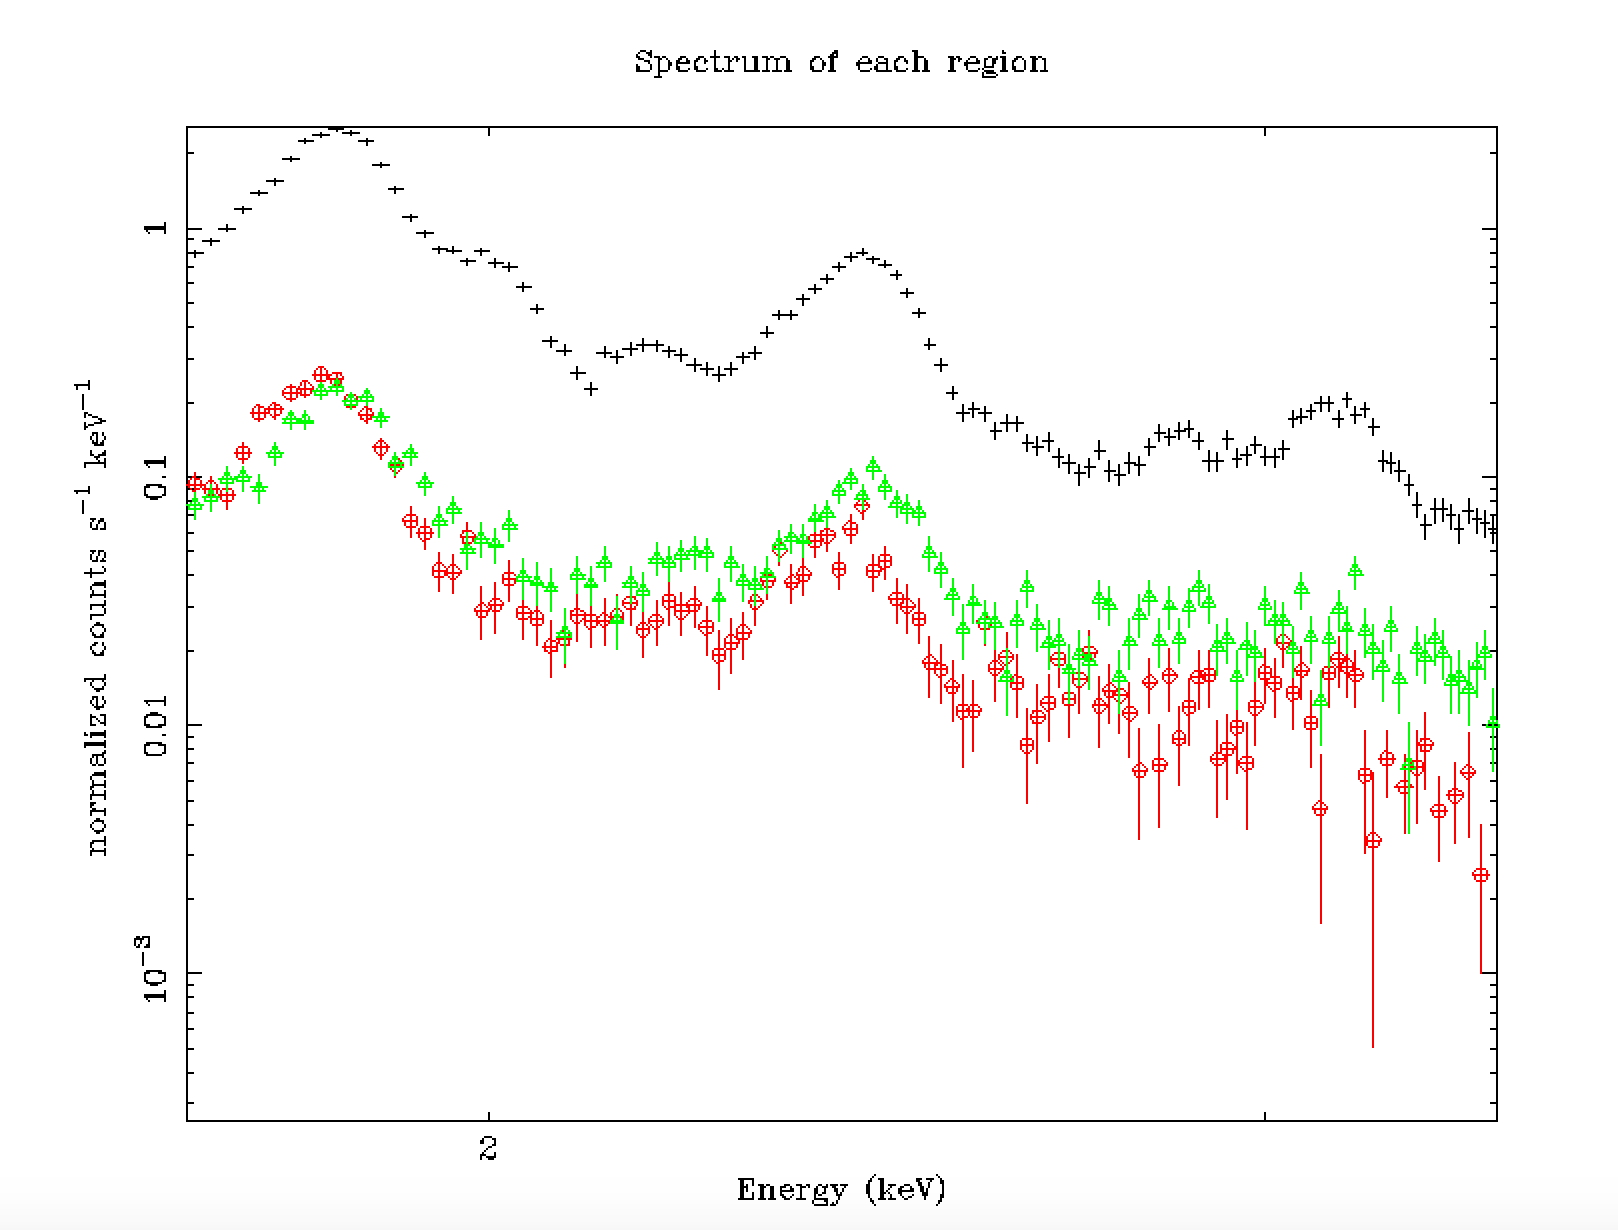
\includegraphics[scale=0.3]{./spectrum_xspec.png}
\end{center}
\end{minipage}
\end{tabular}
\caption{左図:\sf{Chandra}によるG350.1-0.3のフラックスイメージ$\rm{(0.5-8.0~keV)}$、右図:\sf{Chandra}による\sf{SNR}の各領域のスペクトル$\rm{(1.7-3.4~keV)}$ 黒線(マーカー:$+$):東側のスペクトル、赤線($\bigcirc$):南側のスペクトル、緑線($\bigtriangleup$):北側のスペクトル}
\label{fig:spec_reg}
\end{center}
\end{figure}

これらのスペクトルをイジェクタのアバンダンスを確かめるために\textrm{tbabs$\times$vnei}、ドップラーシフトの検証のために\textrm{tbabs$\times$(brems$+$gaussian)}と\textrm{tbabs$\times$(brems$+$zgaussian)}を用いて、解析を行った。\\
それぞれの領域のスペクトルをFig.{}、解析結果をtable.{}に示す。
\begin{figure}[H]
\begin{center}
\begin{tabular}{cc}

\begin{minipage}{0.5\hsize}
\begin{center}
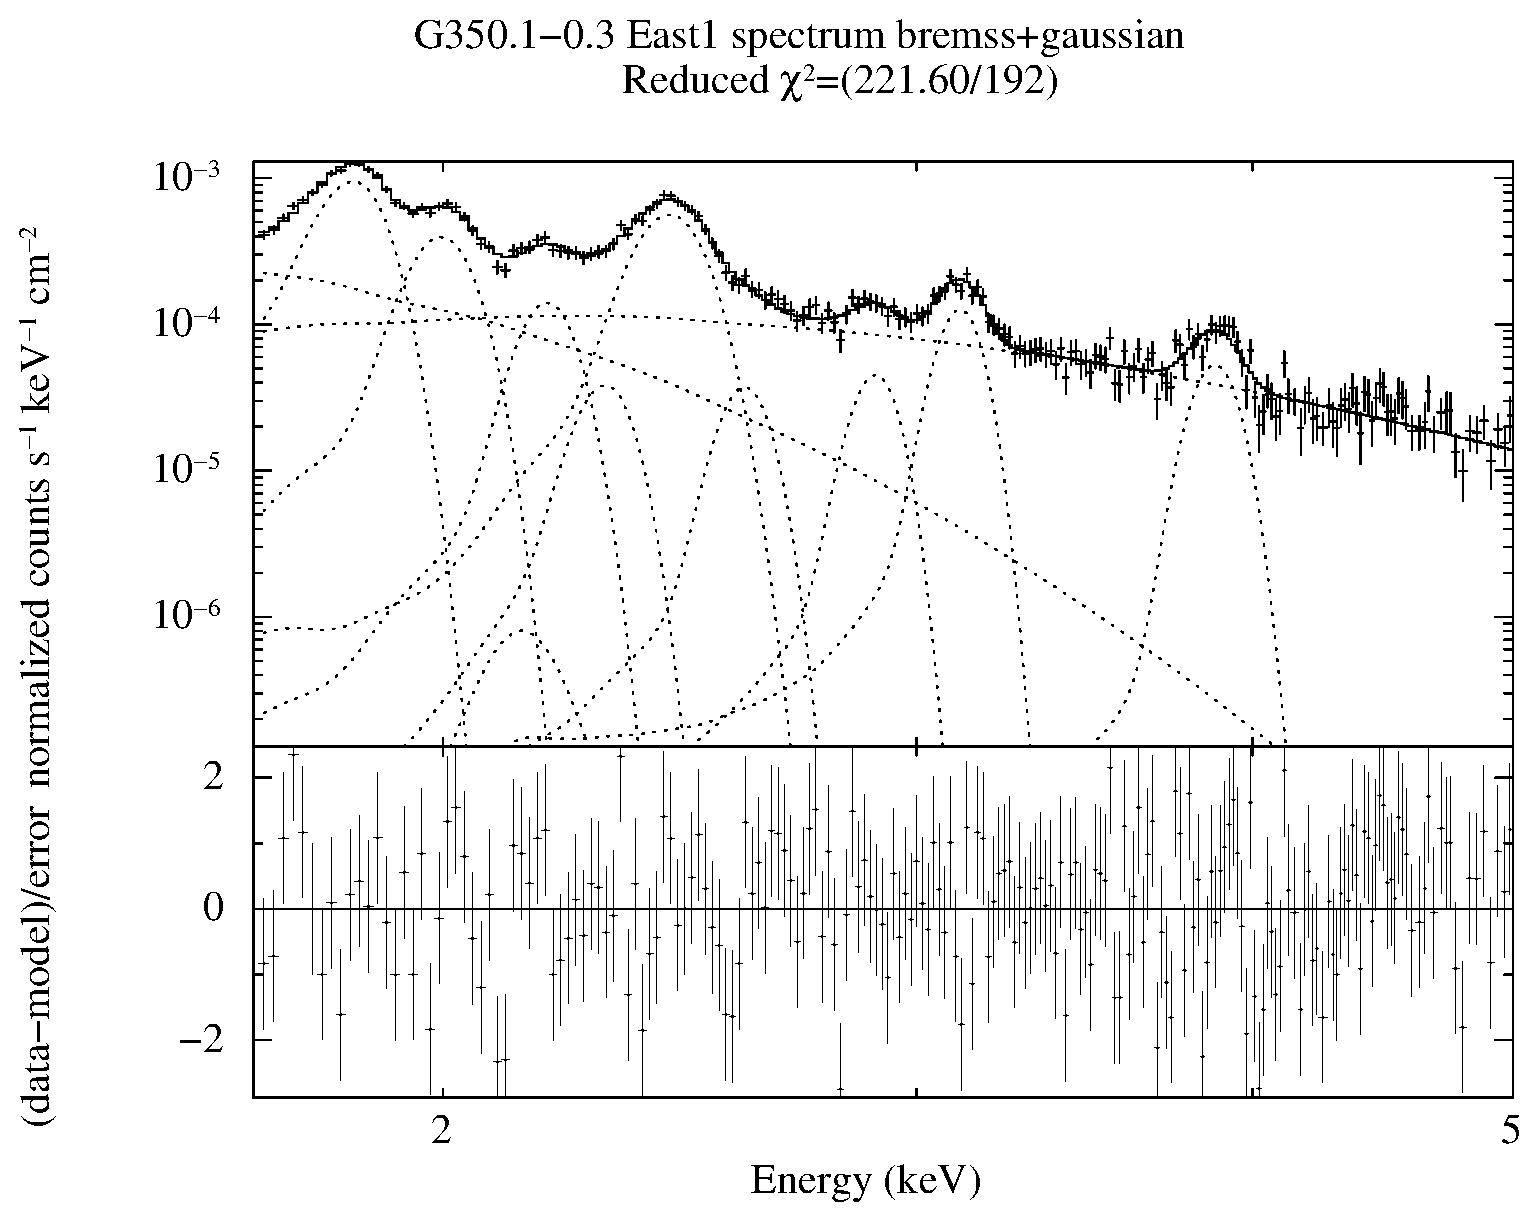
\includegraphics[scale=0.30]{./ps/East1_bremss+gaussian.eps}
\end{center}
\end{minipage}

\begin{minipage}{0.5\hsize}
\begin{center}
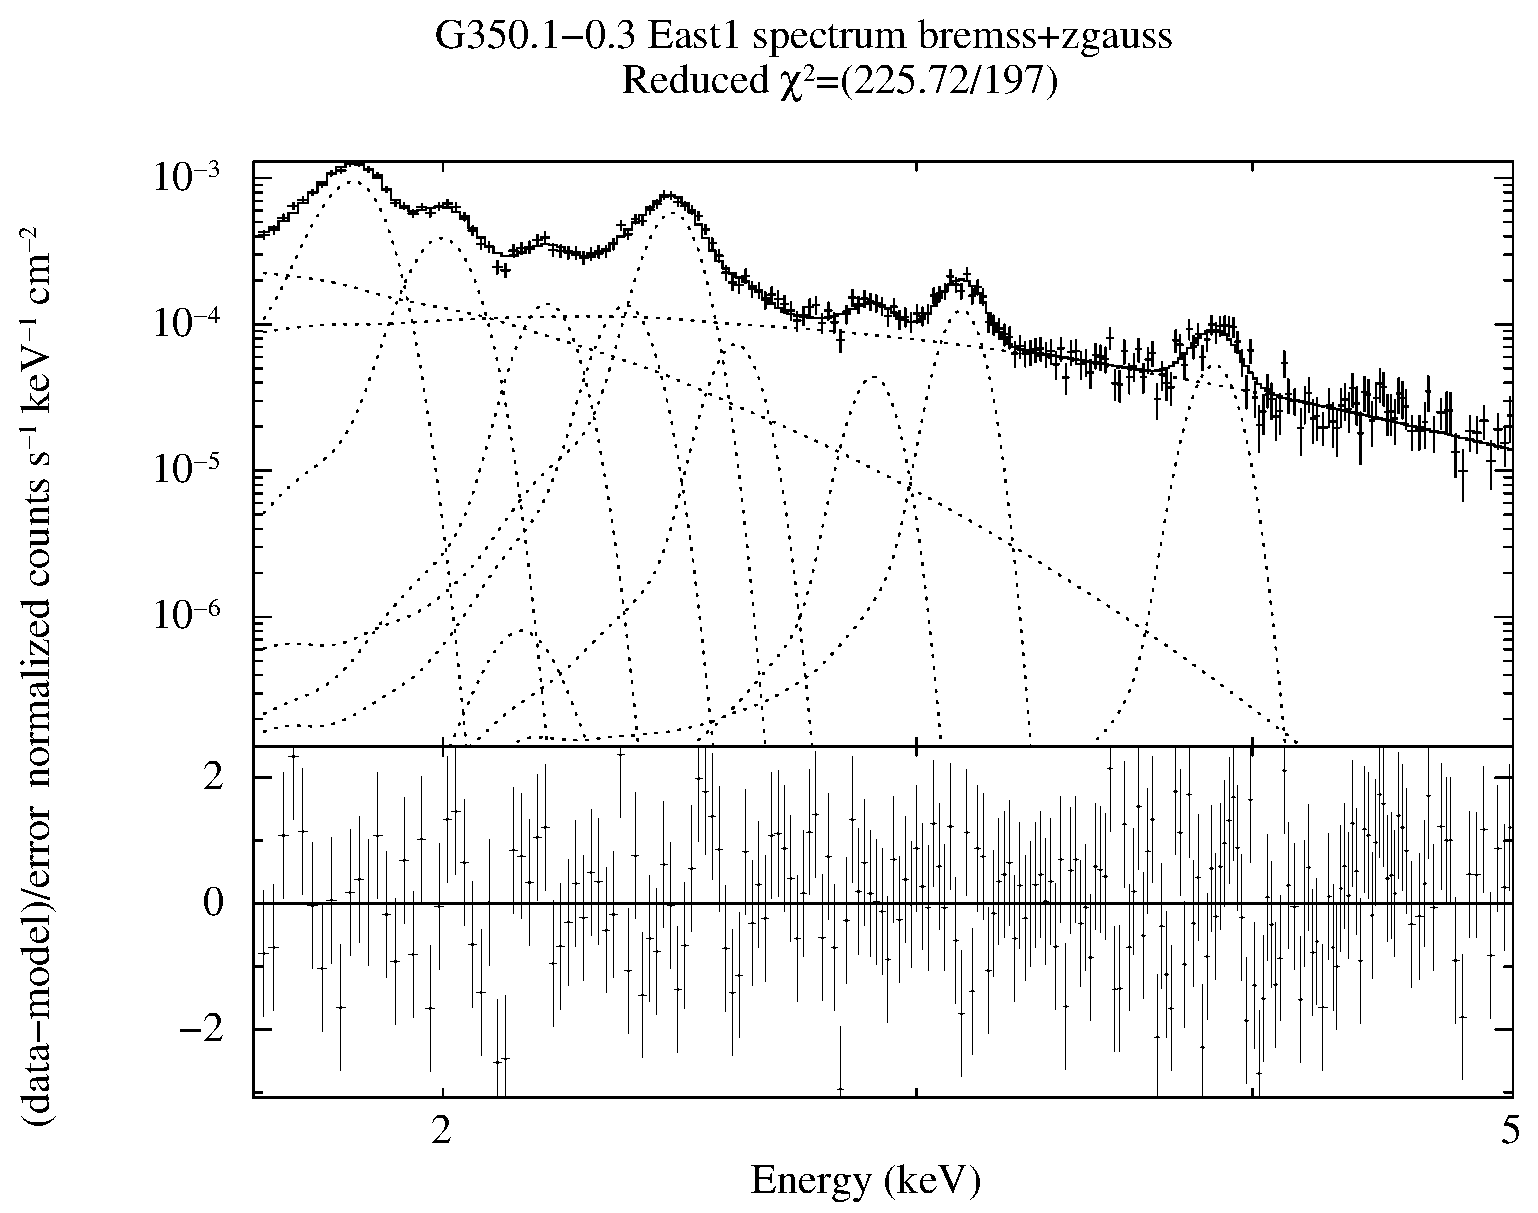
\includegraphics[scale=0.30]{./ps/East1_bremss+zgaussian.eps}
\end{center}
\end{minipage}
\end{tabular}
\caption{左図:East1領域をtbabs$\times$(bremss+gaussian)を用いてフィッティングを行なったスペクトルとモデルとの$\chi$の値、右図:East1領域をtbabs$\times$(bremss+zgaussian)を用いてフィッティングを行なったスペクトルとモデルとの$\chi$の値}
\label{fig:brem_East2}
\end{center}
\end{figure}

\begin{figure}[H]
\begin{center}
\begin{tabular}{cc}

\begin{minipage}{0.5\hsize}
\begin{center}
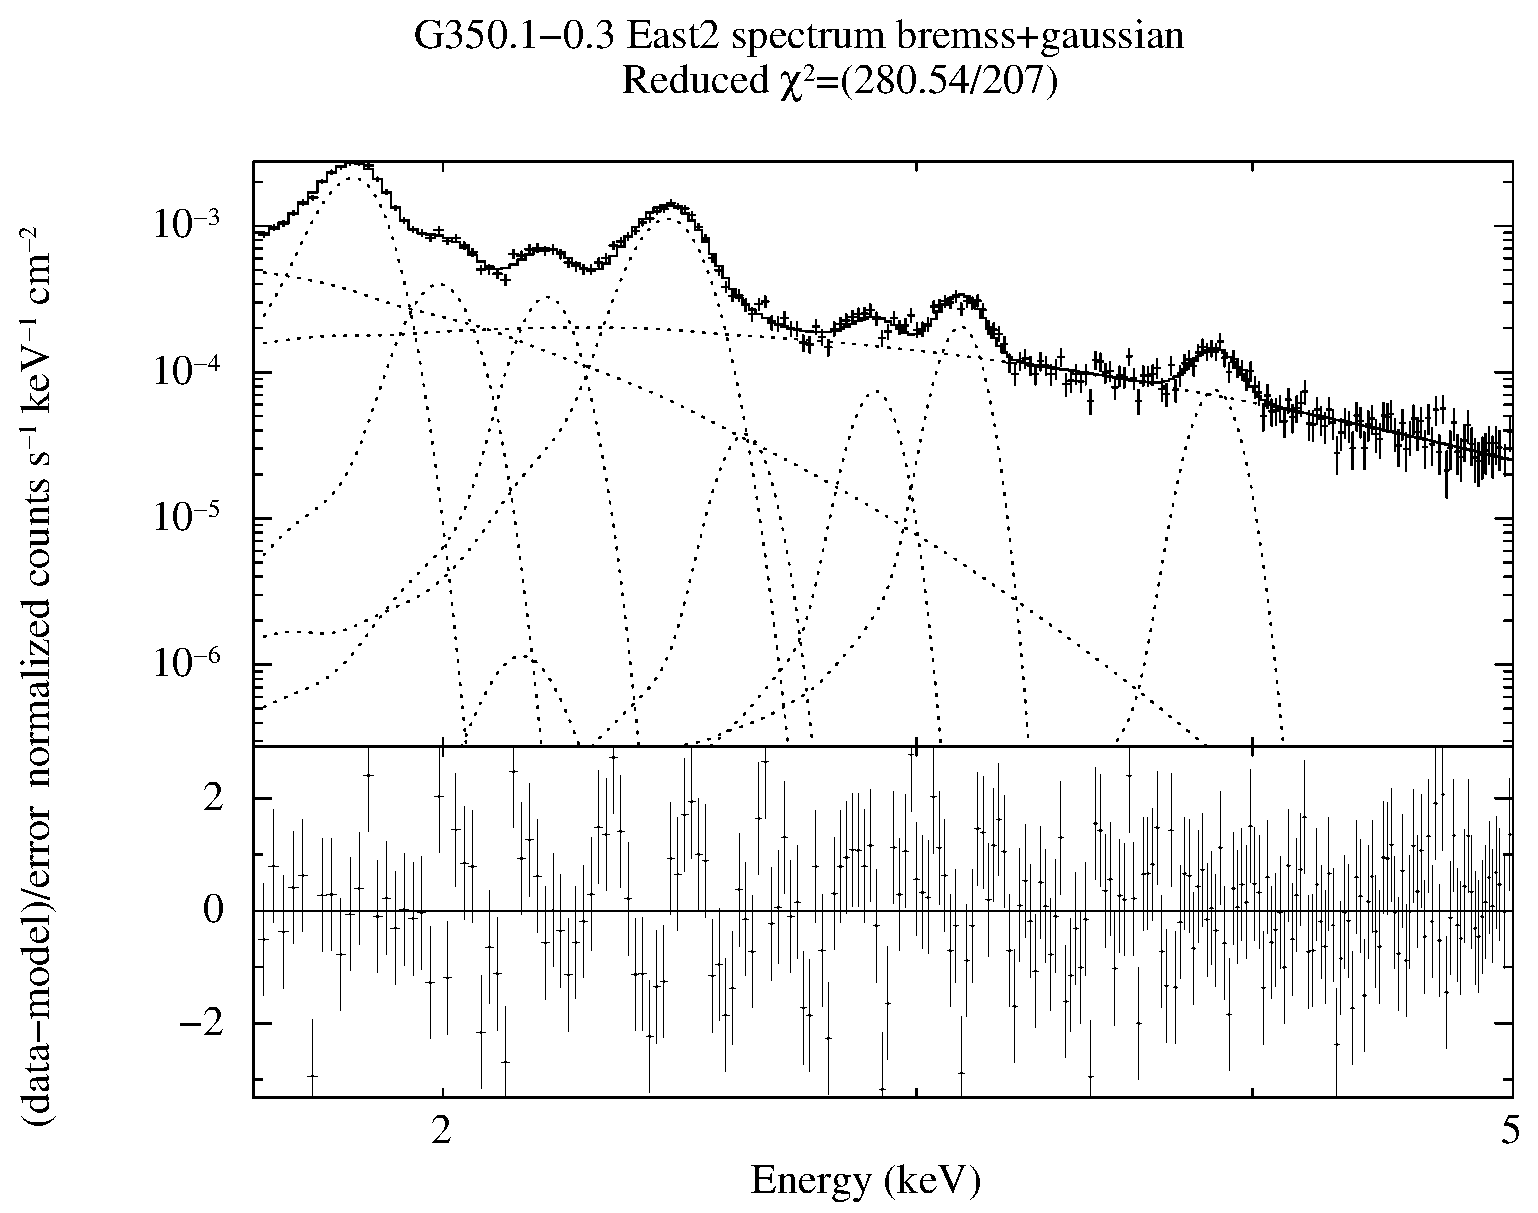
\includegraphics[scale=0.30]{./ps/East2_bremss+gaussian.eps}
\end{center}
\end{minipage}

\begin{minipage}{0.5\hsize}
\begin{center}
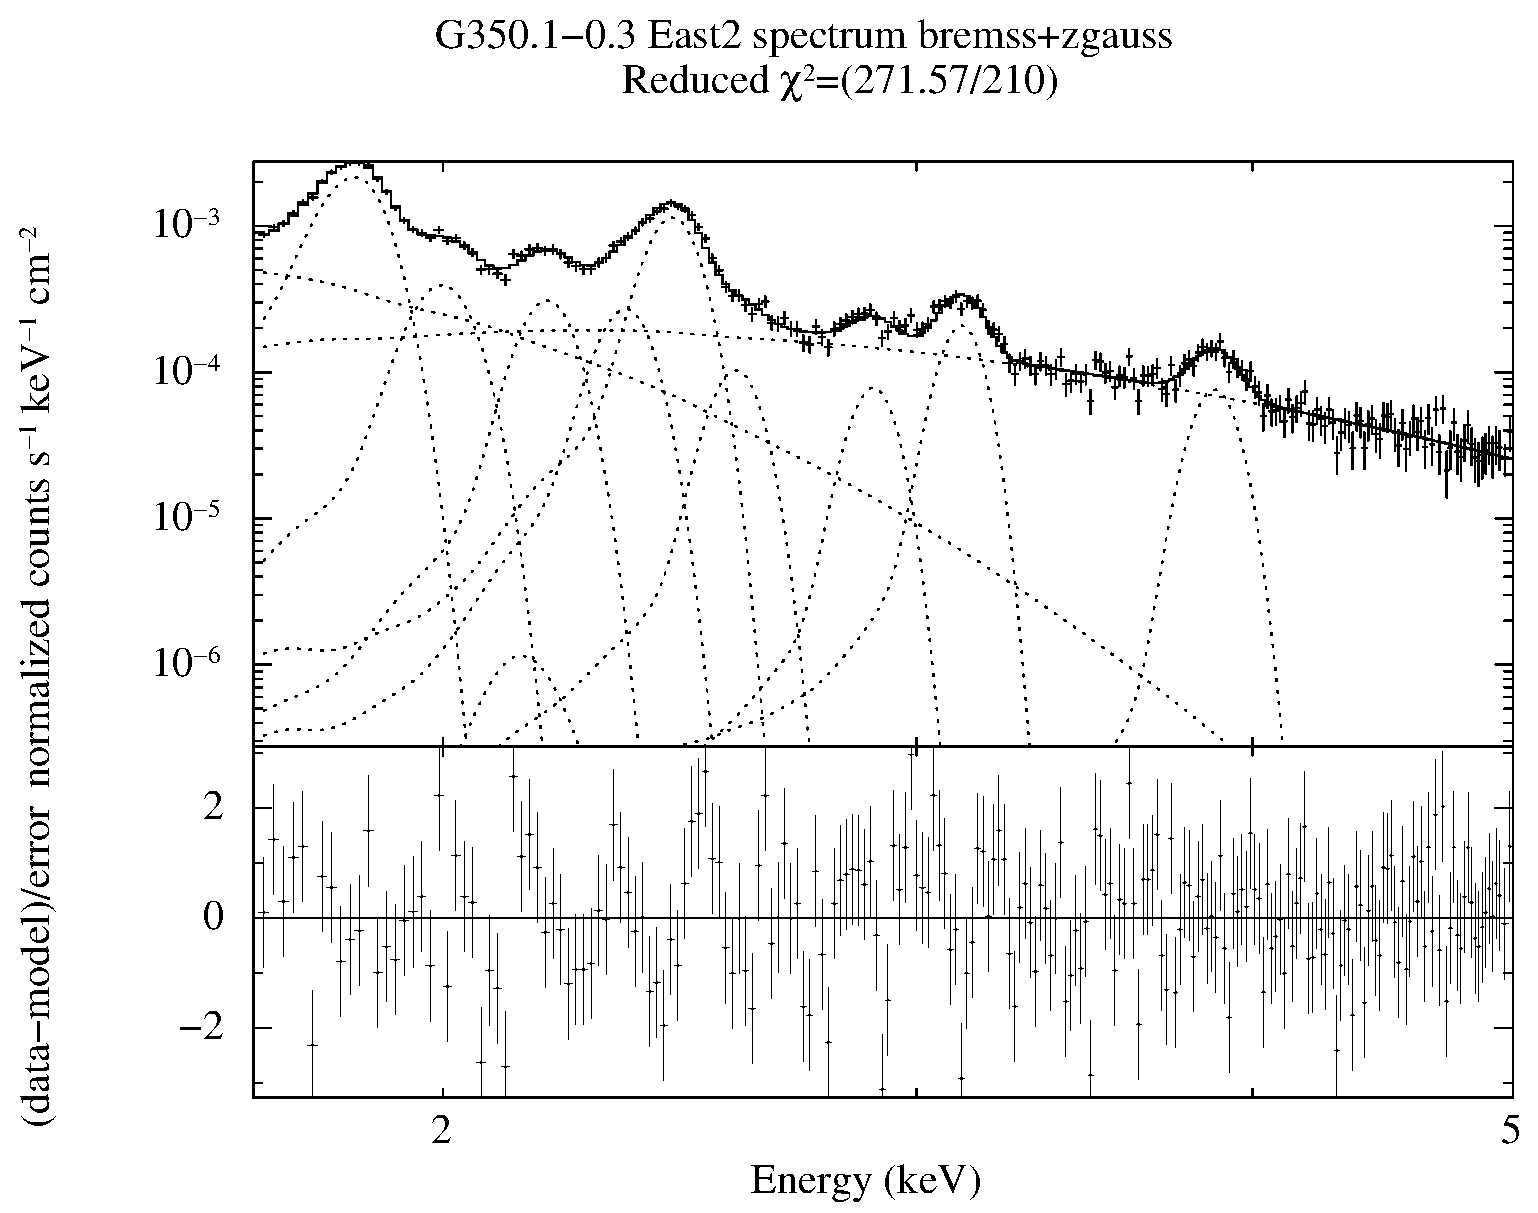
\includegraphics[scale=0.30]{./ps/East2_bremss+zgaussian.eps}
\end{center}
\end{minipage}
\end{tabular}
\caption{左図:East2領域をtbabs$\times$(bremss+gaussian)を用いてフィッティングを行なったスペクトルとモデルとの$\chi$の値、右図:East2領域をtbabs$\times$(bremss+zgaussian)を用いてフィッティングを行なったスペクトルとモデルとの$\chi$の値}
\label{fig:brem_East2}
\end{center}
\end{figure}

\begin{figure}[H]
\begin{center}
\begin{tabular}{cc}

\begin{minipage}{0.5\hsize}
\begin{center}
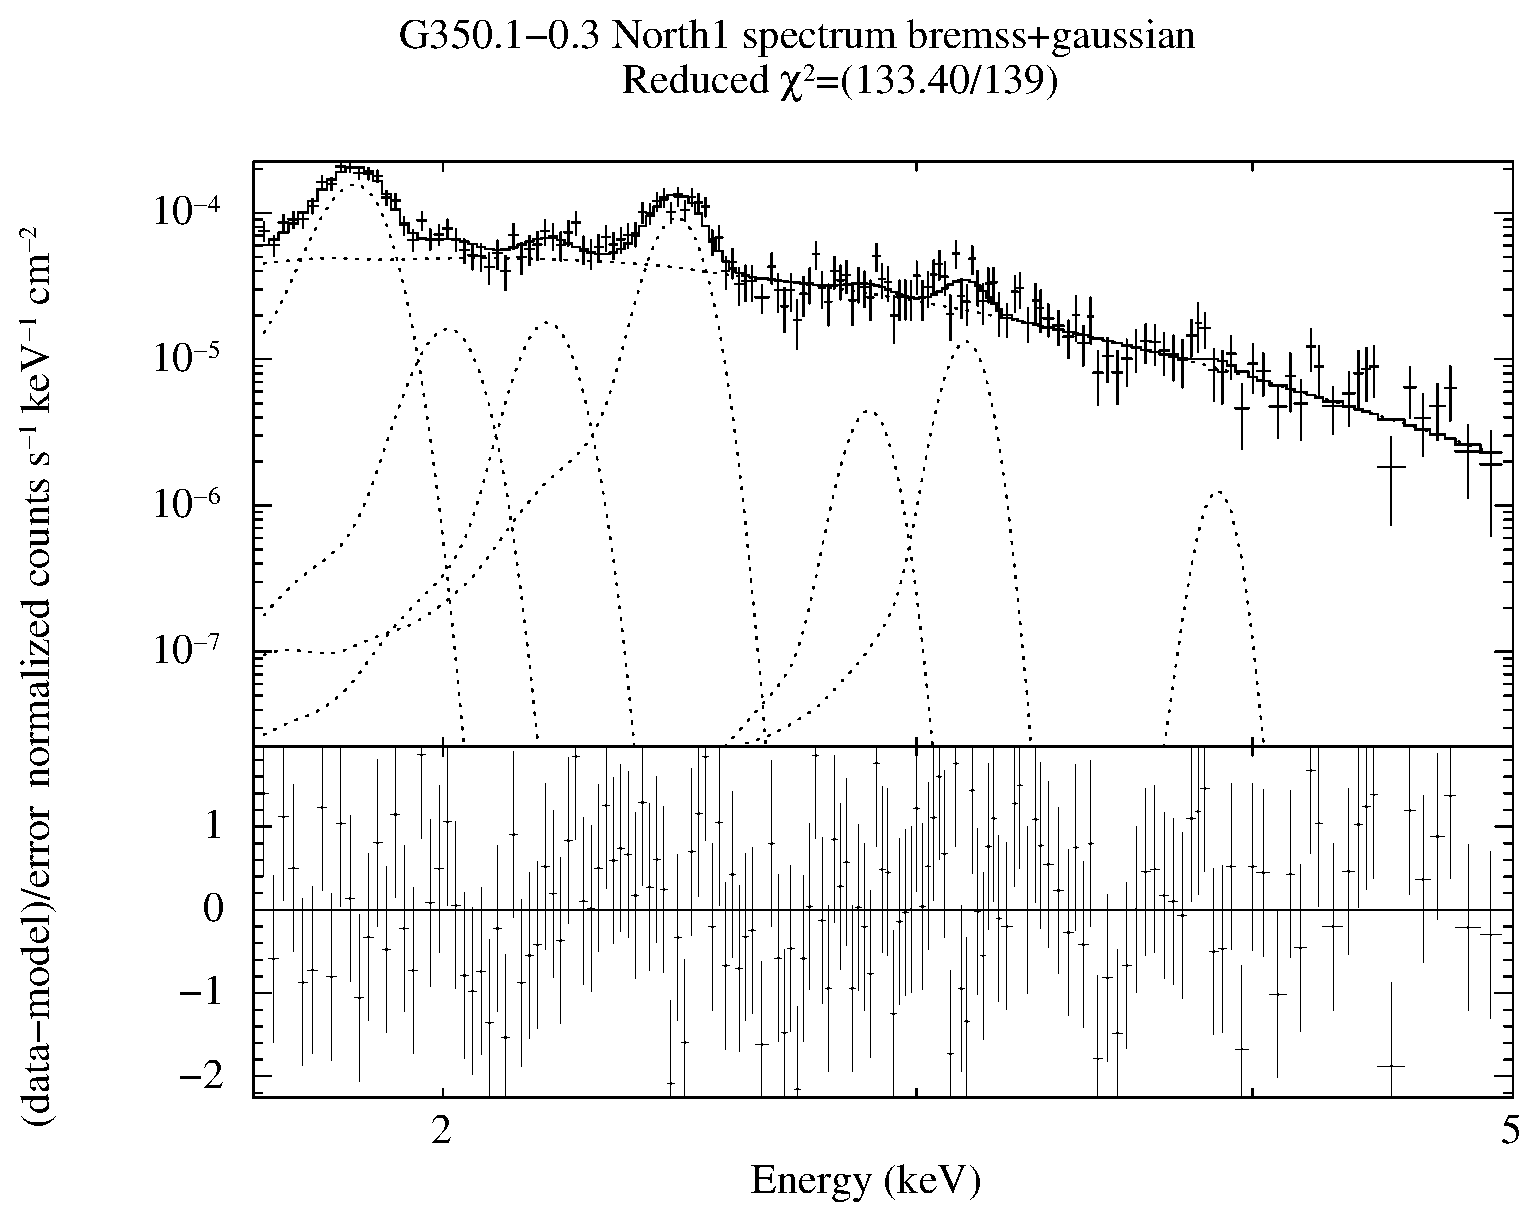
\includegraphics[scale=0.30]{./ps/North1_bremss+gaussian.eps}
\end{center}
\end{minipage}

\begin{minipage}{0.5\hsize}
\begin{center}
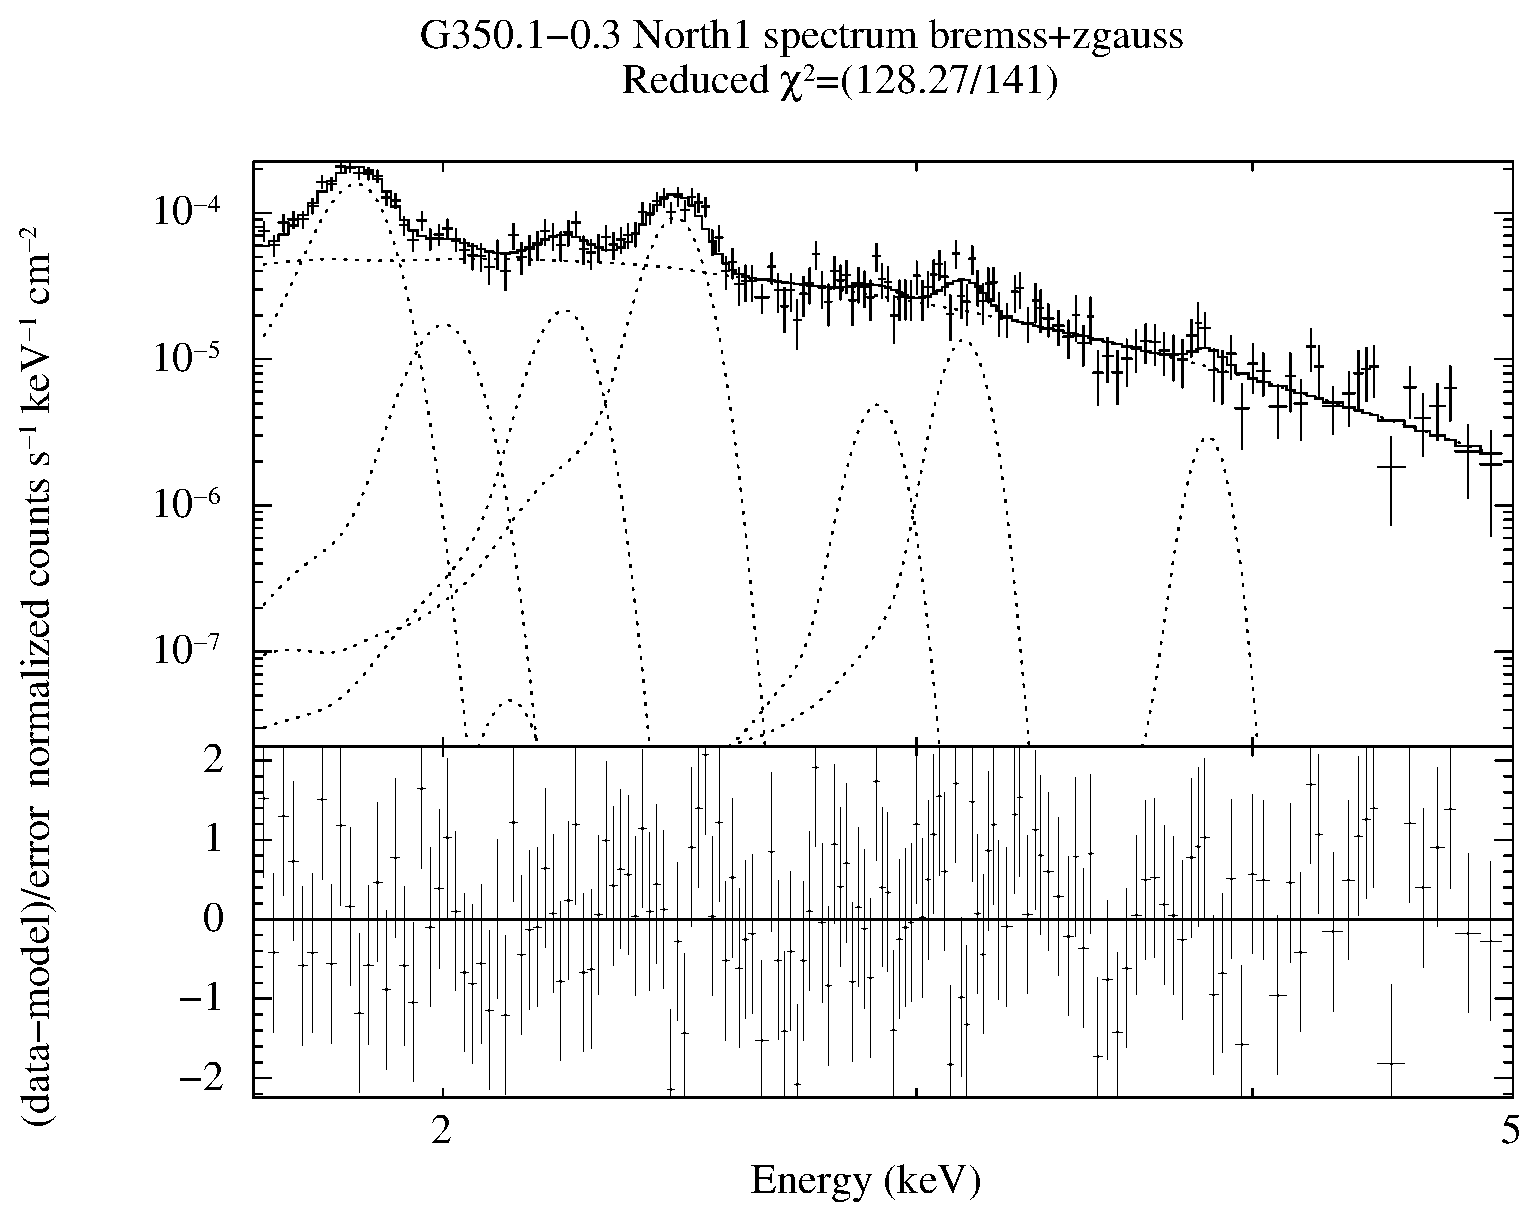
\includegraphics[scale=0.30]{./ps/North1_bremss+zgaussian.eps}
\end{center}
\end{minipage}
\end{tabular}
\caption{左図:North1領域をtbabs$\times$(bremss+gaussian)を用いてフィッティングを行なったスペクトルとモデルとの$\chi$の値、右図:North1領域をtbabs$\times$(bremss+zgaussian)を用いてフィッティングを行なったスペクトルとモデルとの$\chi$の値}
\label{fig:brem_North1}
\end{center}
\end{figure}

\begin{figure}[H]
\begin{center}
\begin{tabular}{cc}

\begin{minipage}{0.5\hsize}
\begin{center}
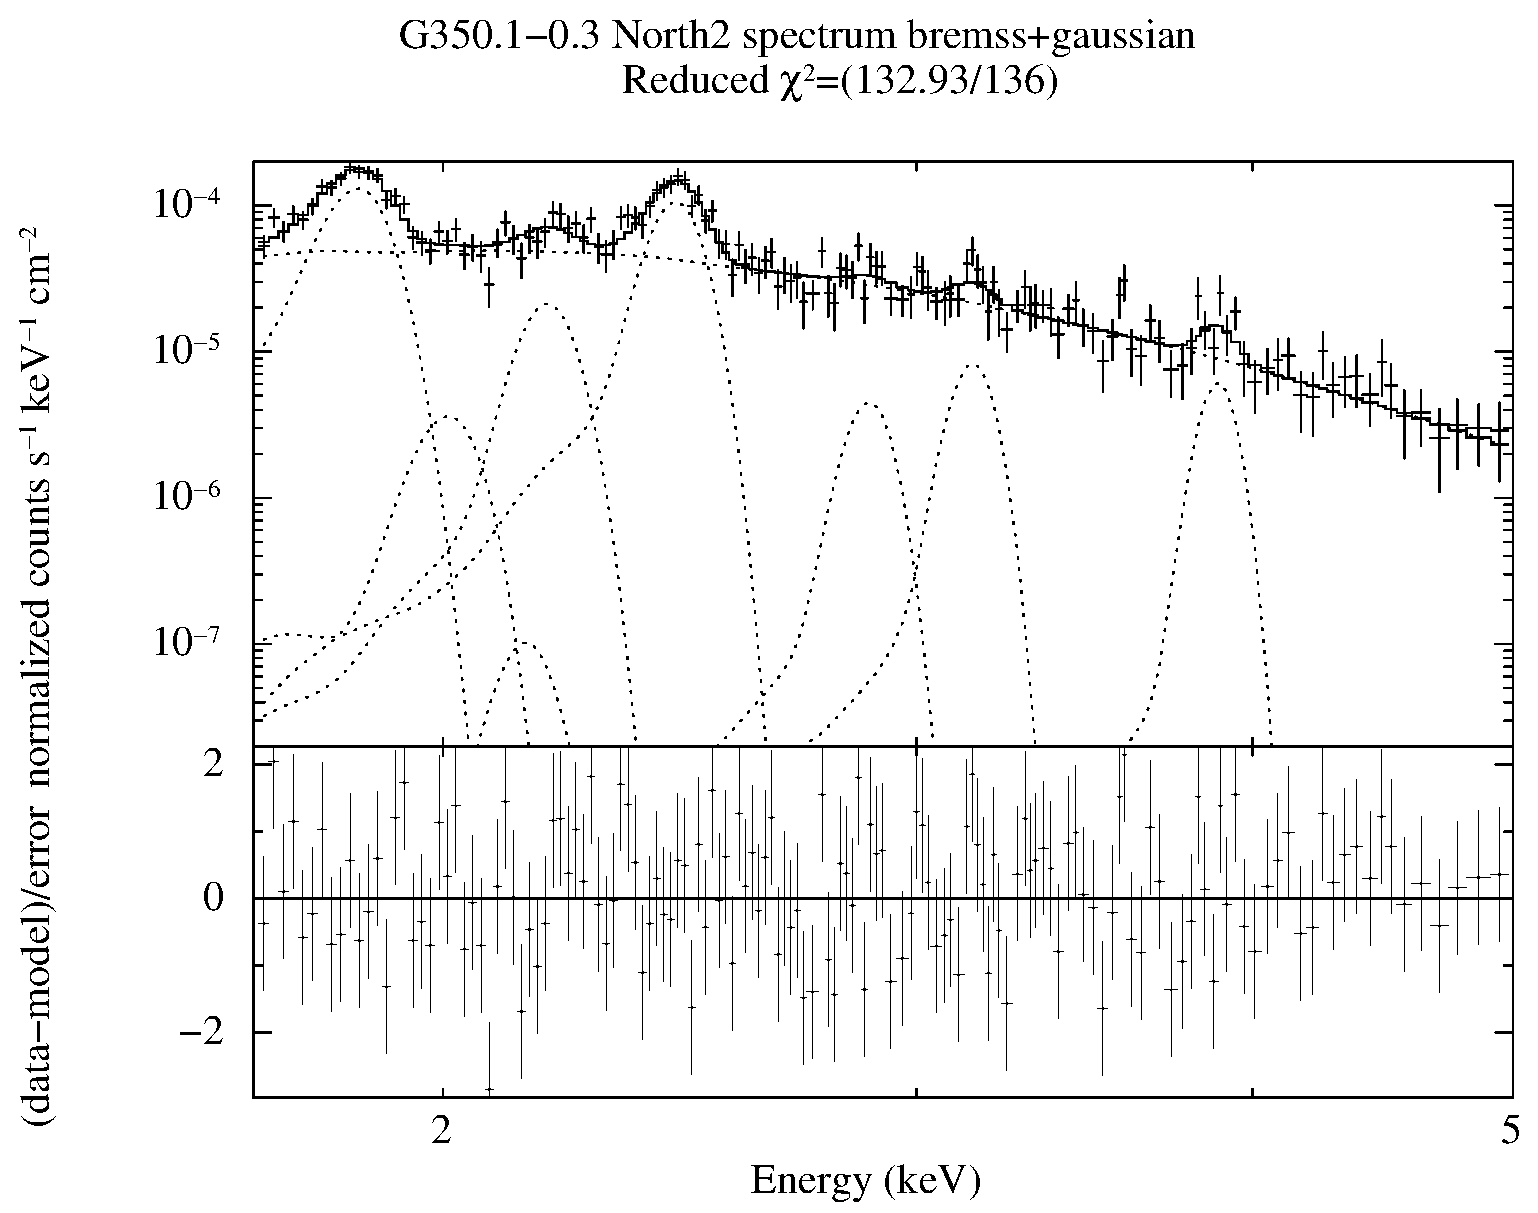
\includegraphics[scale=0.30]{./ps/North2_bremss+gaussian.eps}
\end{center}
\end{minipage}

\begin{minipage}{0.5\hsize}
\begin{center}
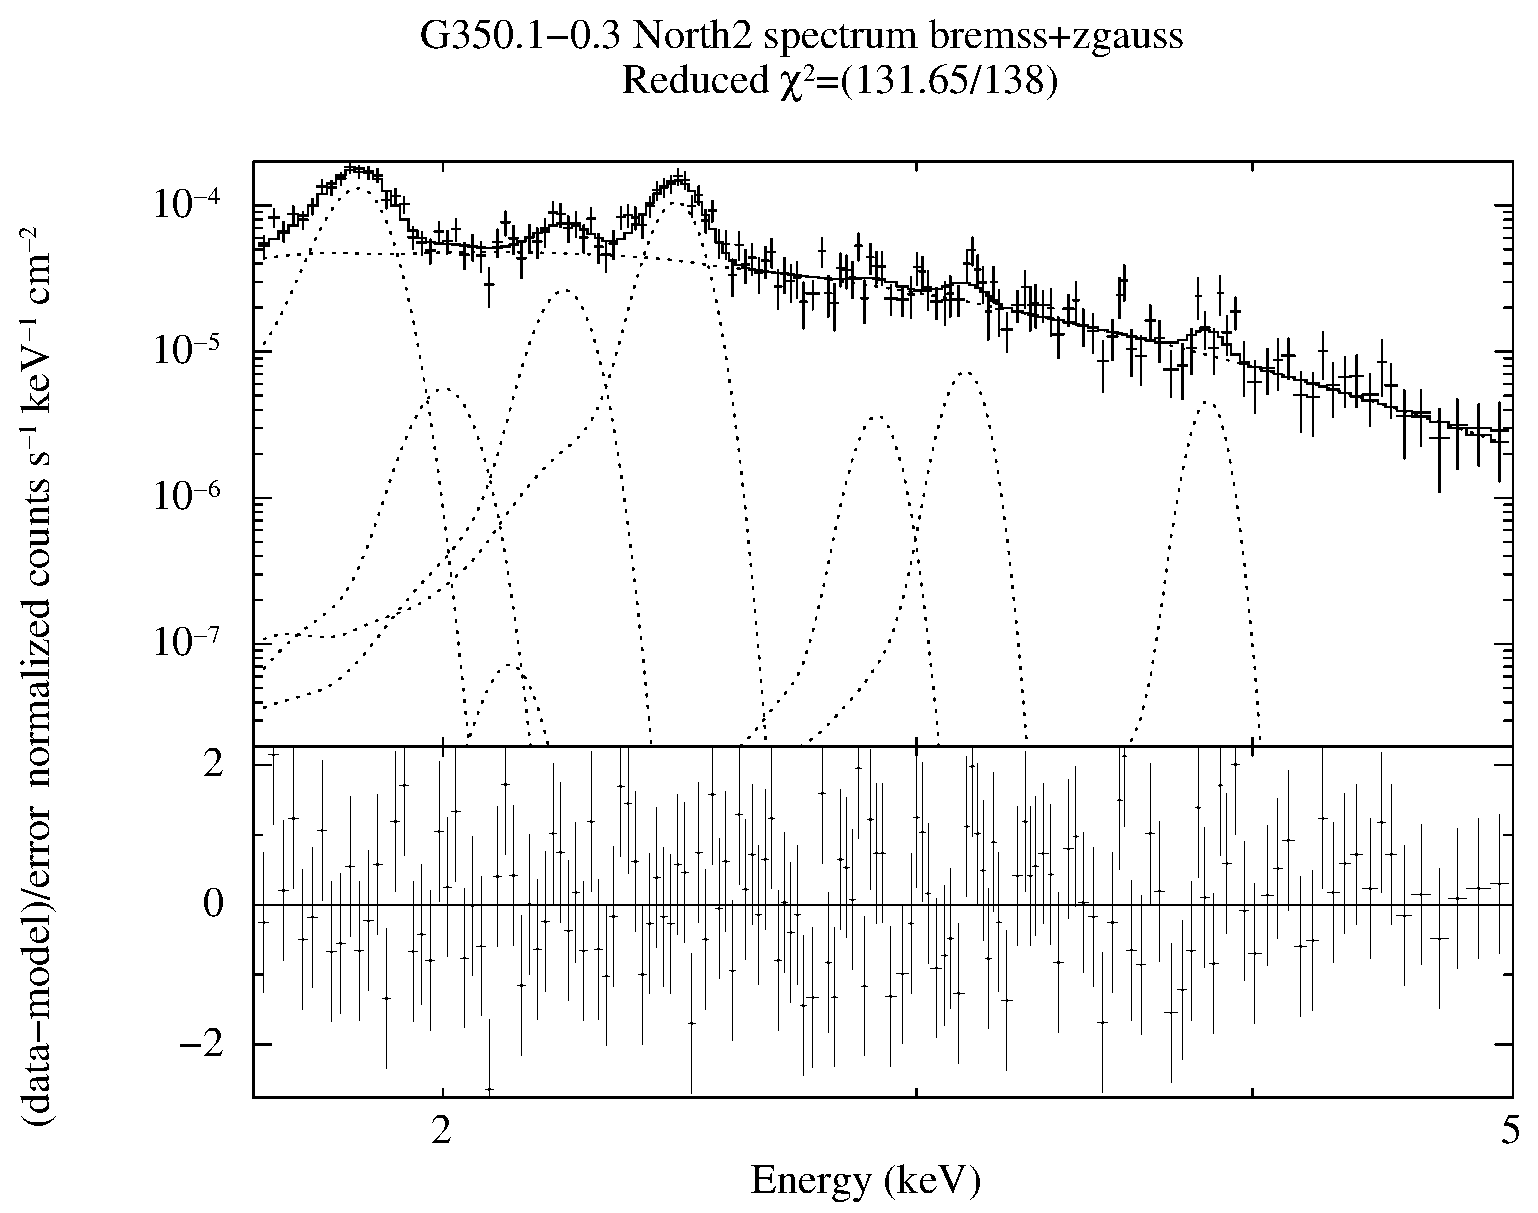
\includegraphics[scale=0.30]{./ps/North2_bremss+zgaussian.eps}
\end{center}
\end{minipage}
\end{tabular}
\caption{左図:North2領域をtbabs$\times$(bremss+gaussian)を用いてフィッティングを行なったスペクトルとモデルとの$\chi$の値、右図:North2領域をtbabs$\times$(bremss+zgaussian)を用いてフィッティングを行なったスペクトルとモデルとの$\chi$の値}
\label{fig:brem_North2}
\end{center}
\end{figure}

\begin{figure}[H]
\begin{center}
\begin{tabular}{cc}

\begin{minipage}{0.5\hsize}
\begin{center}
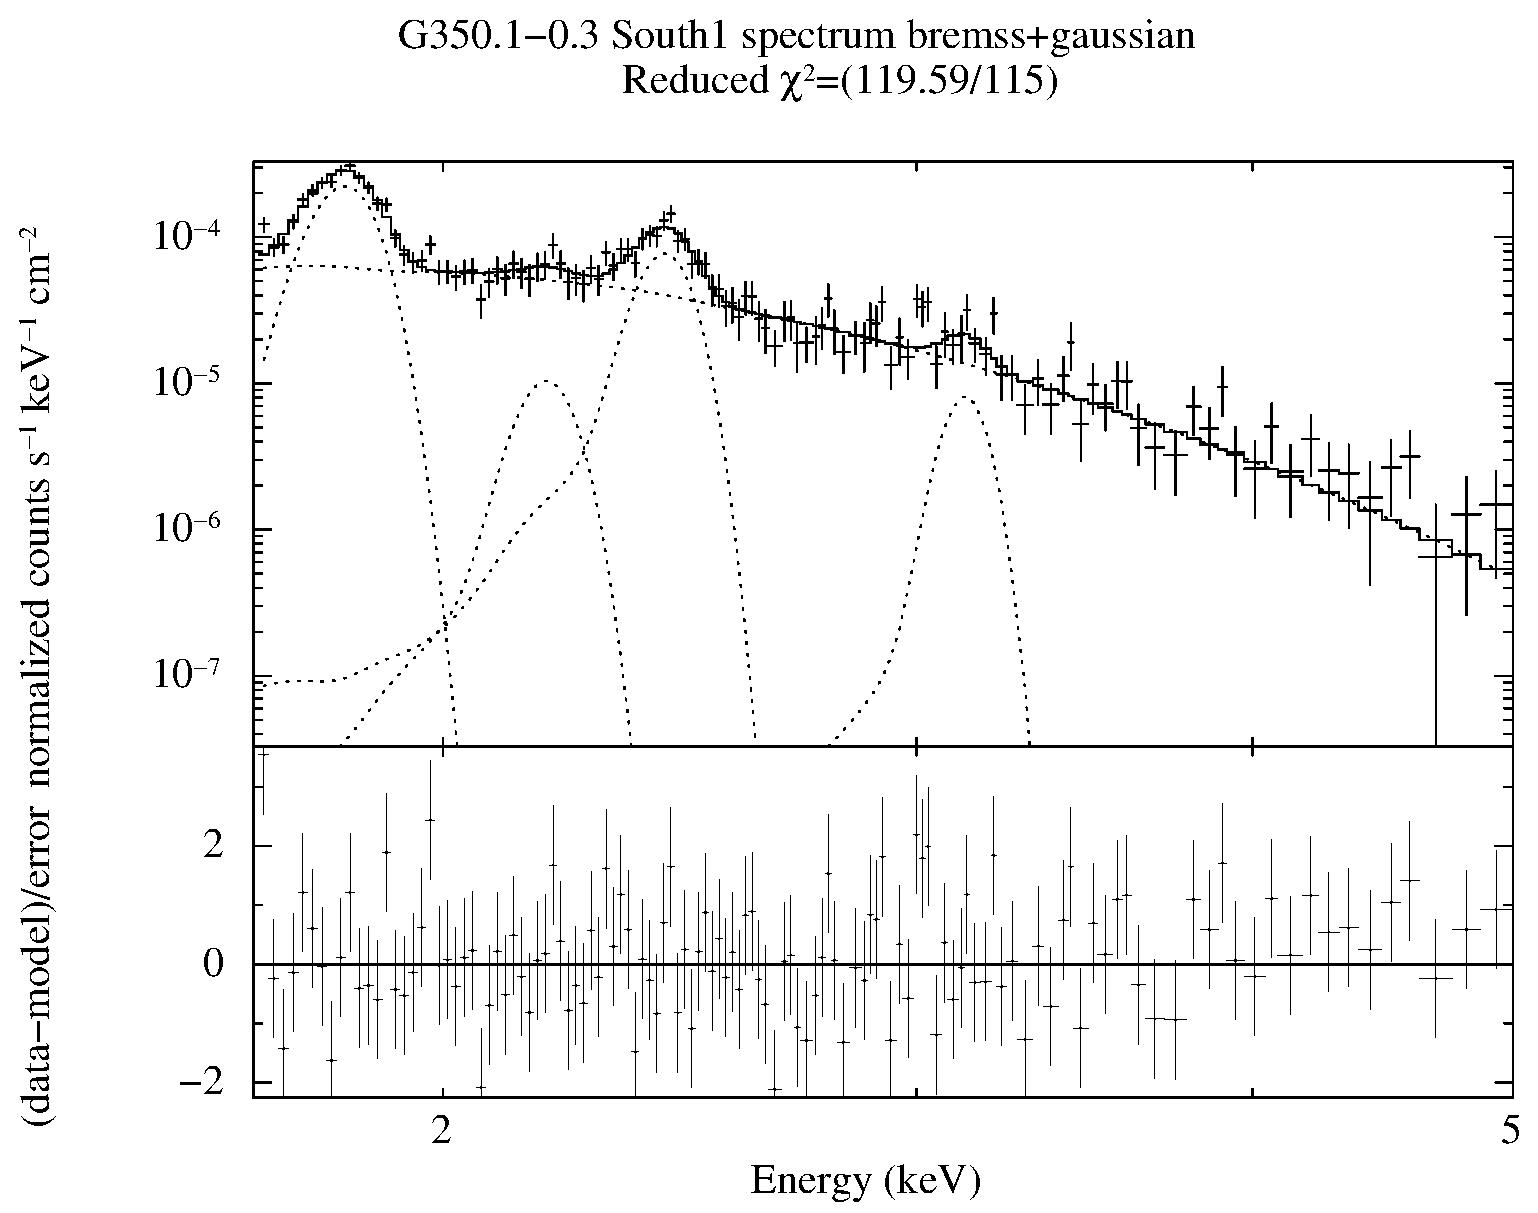
\includegraphics[scale=0.30]{./ps/South1_bremss+gaussian.eps}
\end{center}
\end{minipage}

\begin{minipage}{0.5\hsize}
\begin{center}
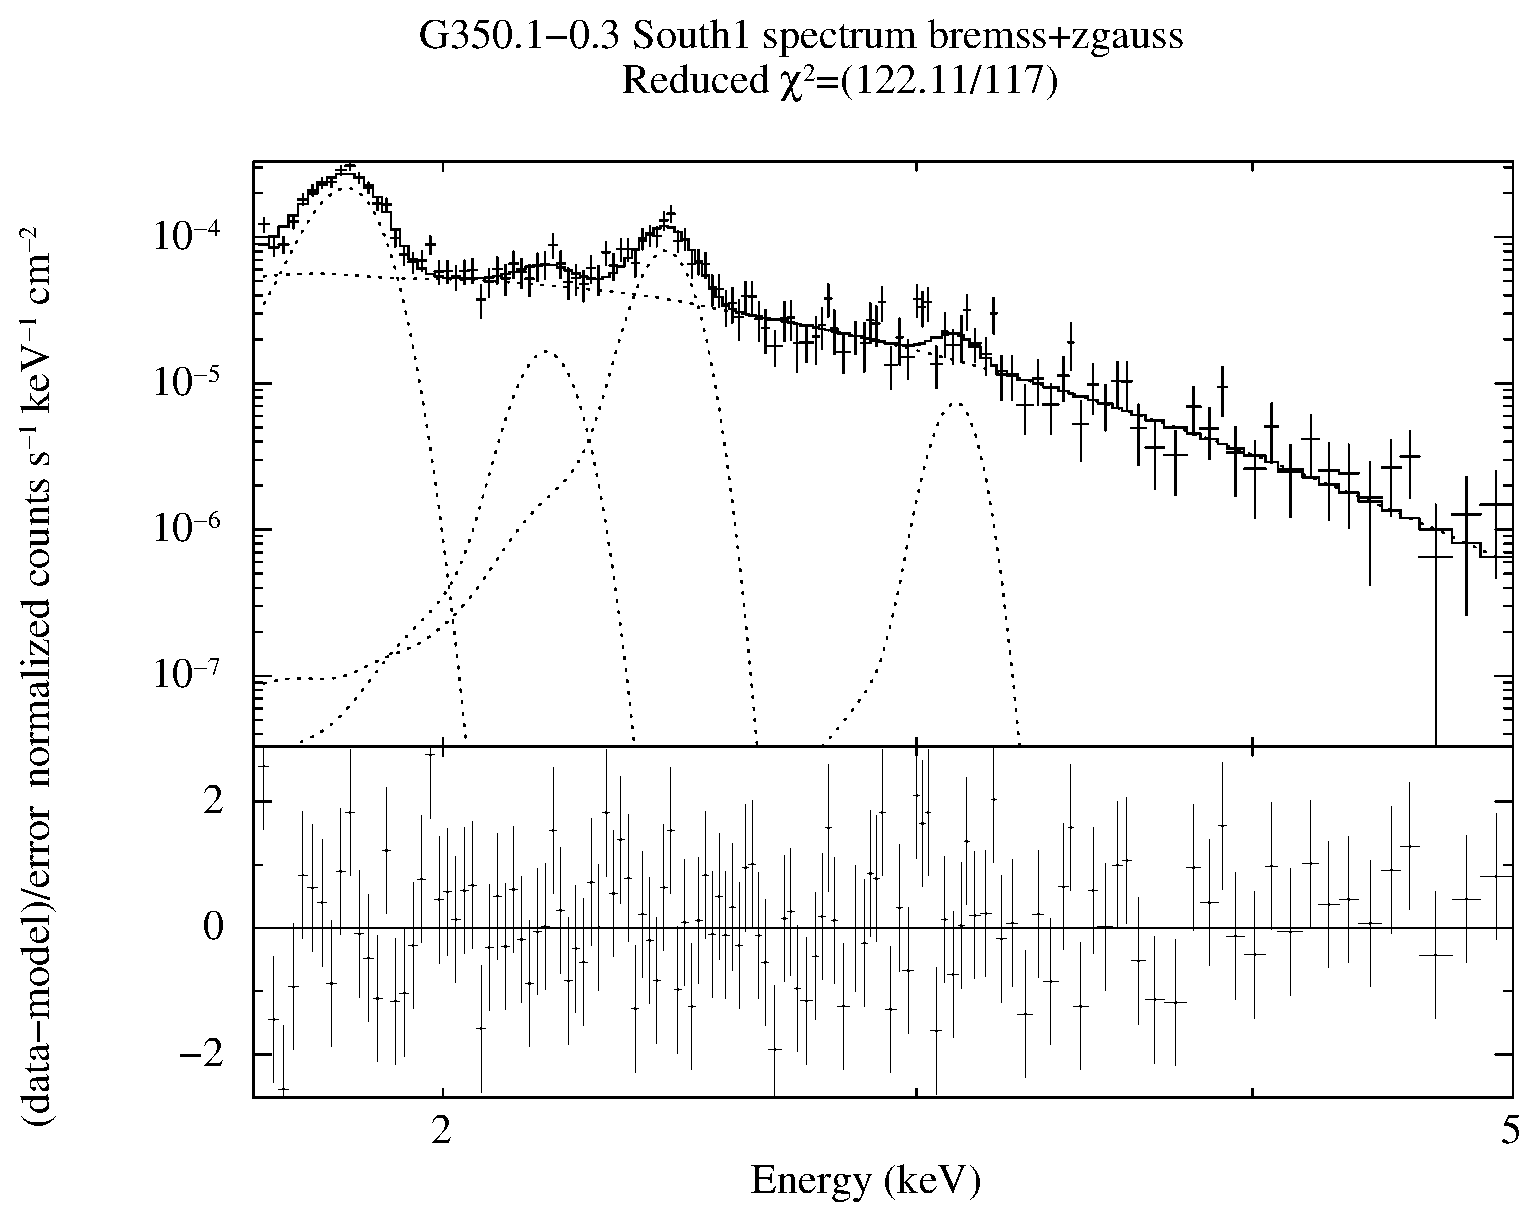
\includegraphics[scale=0.30]{./ps/South1_bremss+zgaussian.eps}
\end{center}
\end{minipage}
\end{tabular}
\caption{左図:South1領域をtbabs$\times$(bremss+gaussian)を用いてフィッティングを行なったスペクトルとモデルとの$\chi$の値、右図:South1領域をtbabs$\times$(bremss+zgaussian)を用いてフィッティングを行なったスペクトルとモデルとの$\chi$の値}
\label{fig:brem_South1}
\end{center}
\end{figure}

\begin{figure}[H]
\begin{center}
\begin{tabular}{cc}

\begin{minipage}{0.5\hsize}
\begin{center}
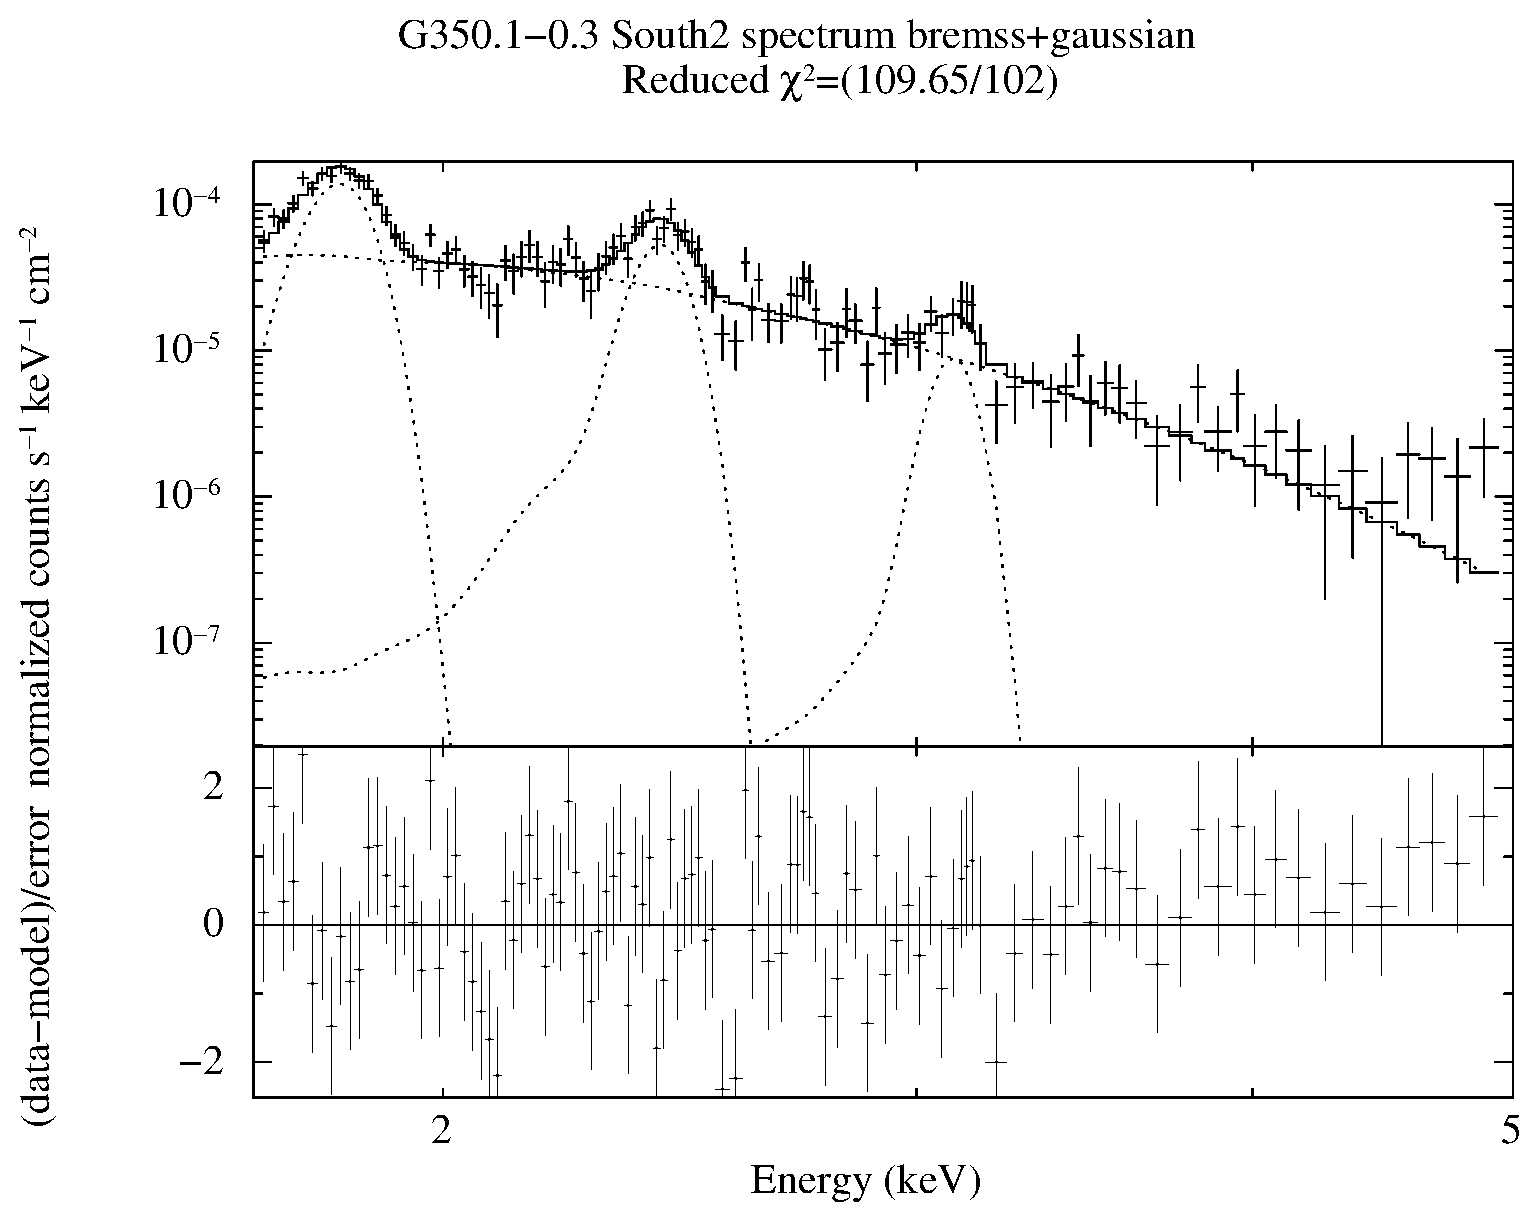
\includegraphics[scale=0.30]{./ps/South2_bremss+gaussian.eps}
\end{center}
\end{minipage}

\begin{minipage}{0.5\hsize}
\begin{center}
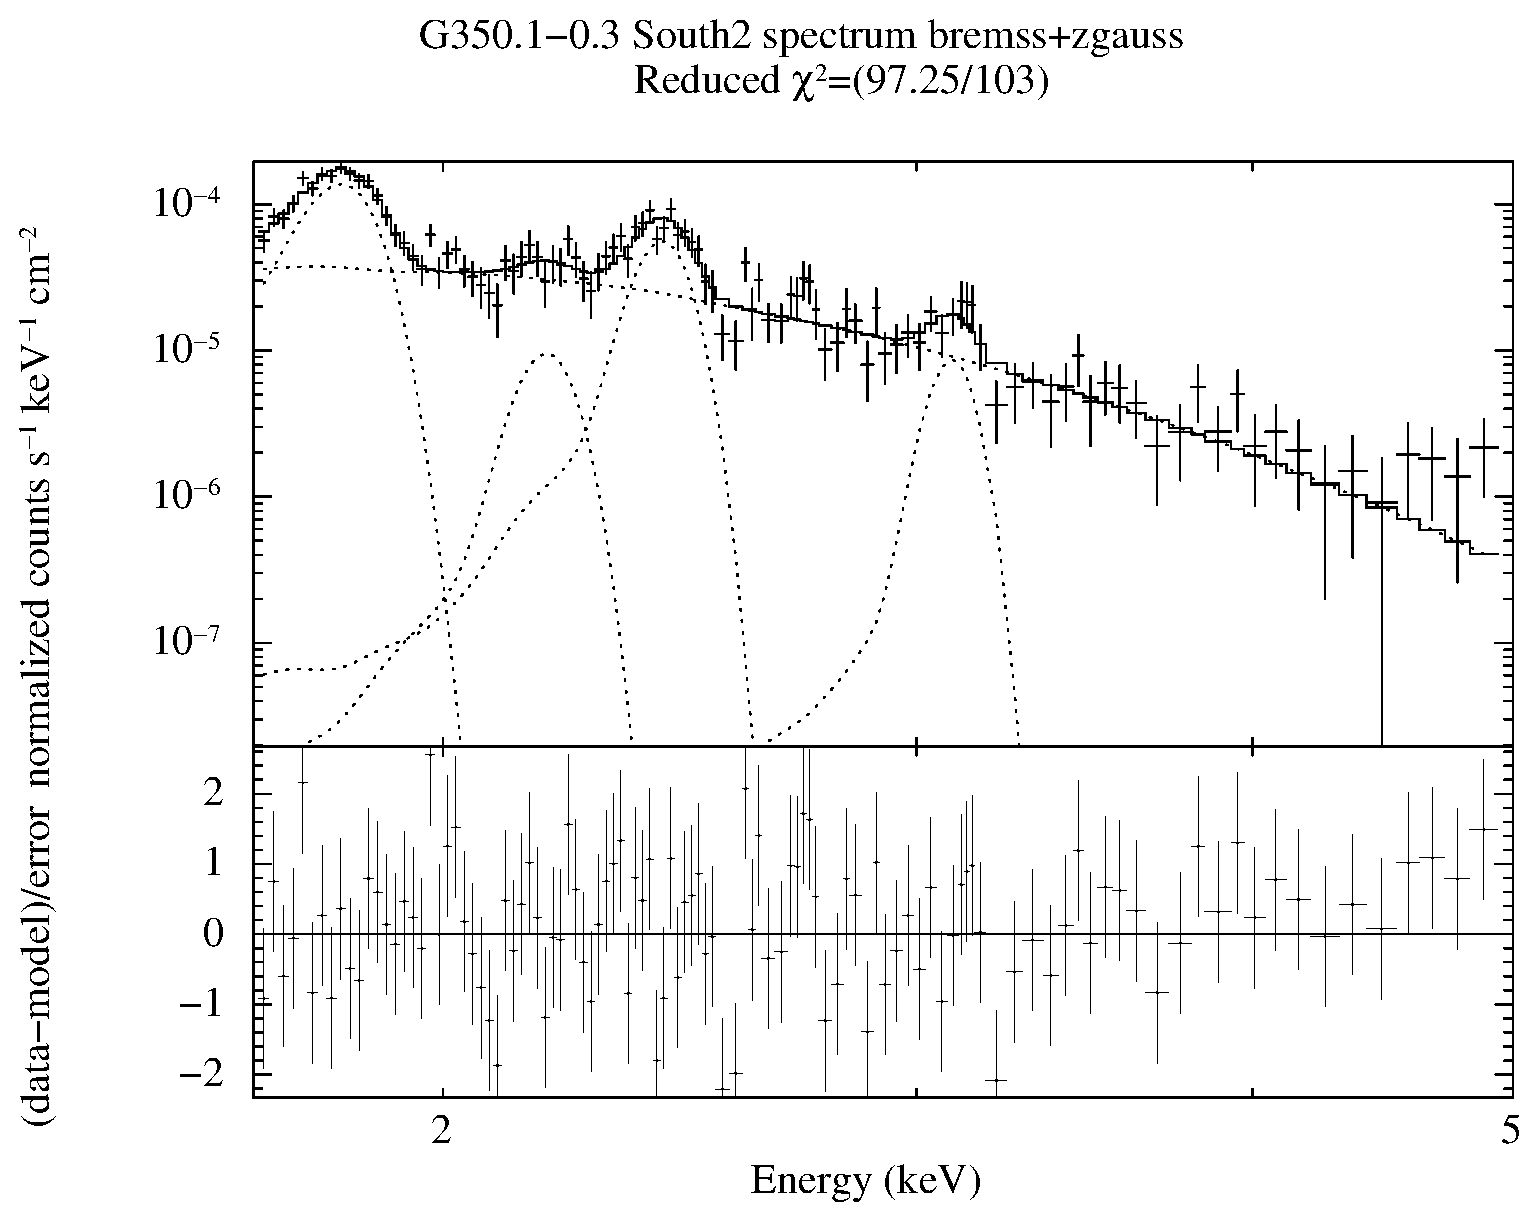
\includegraphics[scale=0.30]{./ps/South2_bremss+zgaussian.eps}
\end{center}
\end{minipage}
\end{tabular}
\caption{左図:South2領域をtbabs$\times$(bremss+gaussian)を用いてフィッティングを行なったスペクトルとモデルとの$\chi$の値、右図:South2領域をtbabs$\times$(bremss+zgaussian)を用いてフィッティングを行なったスペクトルとモデルとの$\chi$の値}
\label{fig:brem_South2}
\end{center}
\end{figure}

\begin{figure}[H]
\begin{center}
\begin{tabular}{cc}

\begin{minipage}{0.5\hsize}
\begin{center}
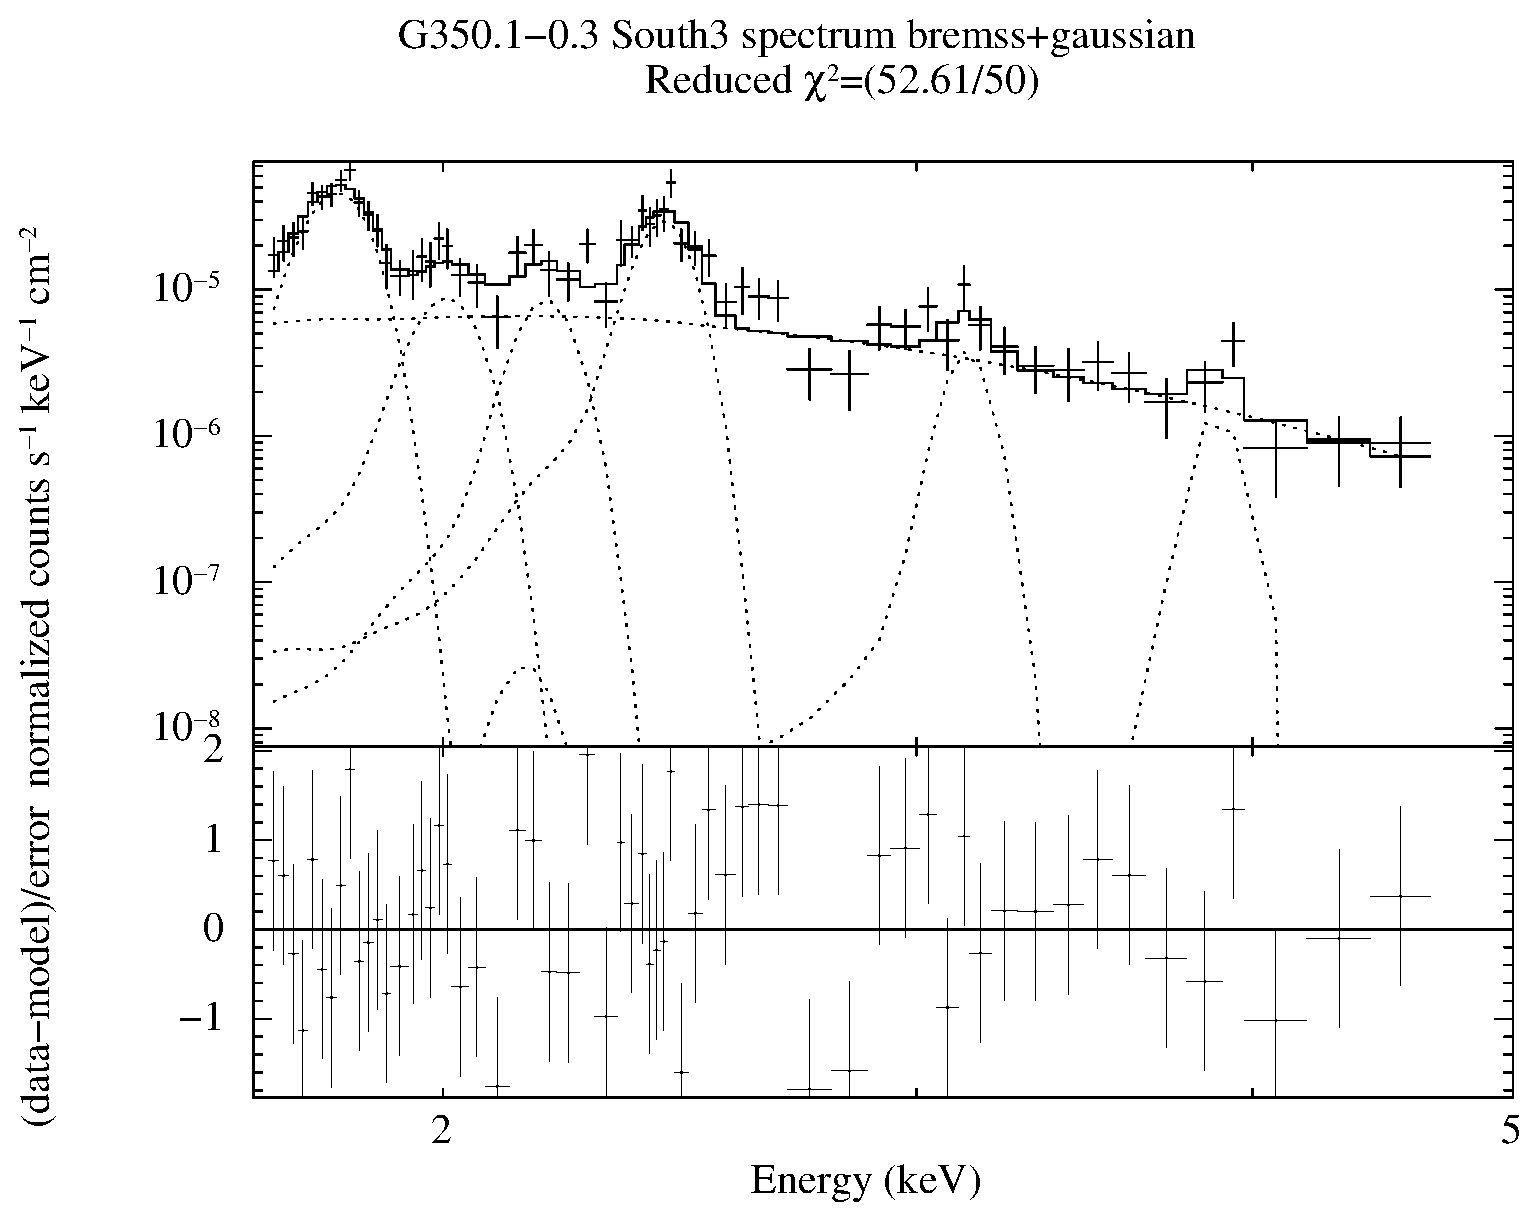
\includegraphics[scale=0.30]{./ps/South3_bremss+gaussian.eps}
\end{center}
\end{minipage}

\begin{minipage}{0.5\hsize}
\begin{center}
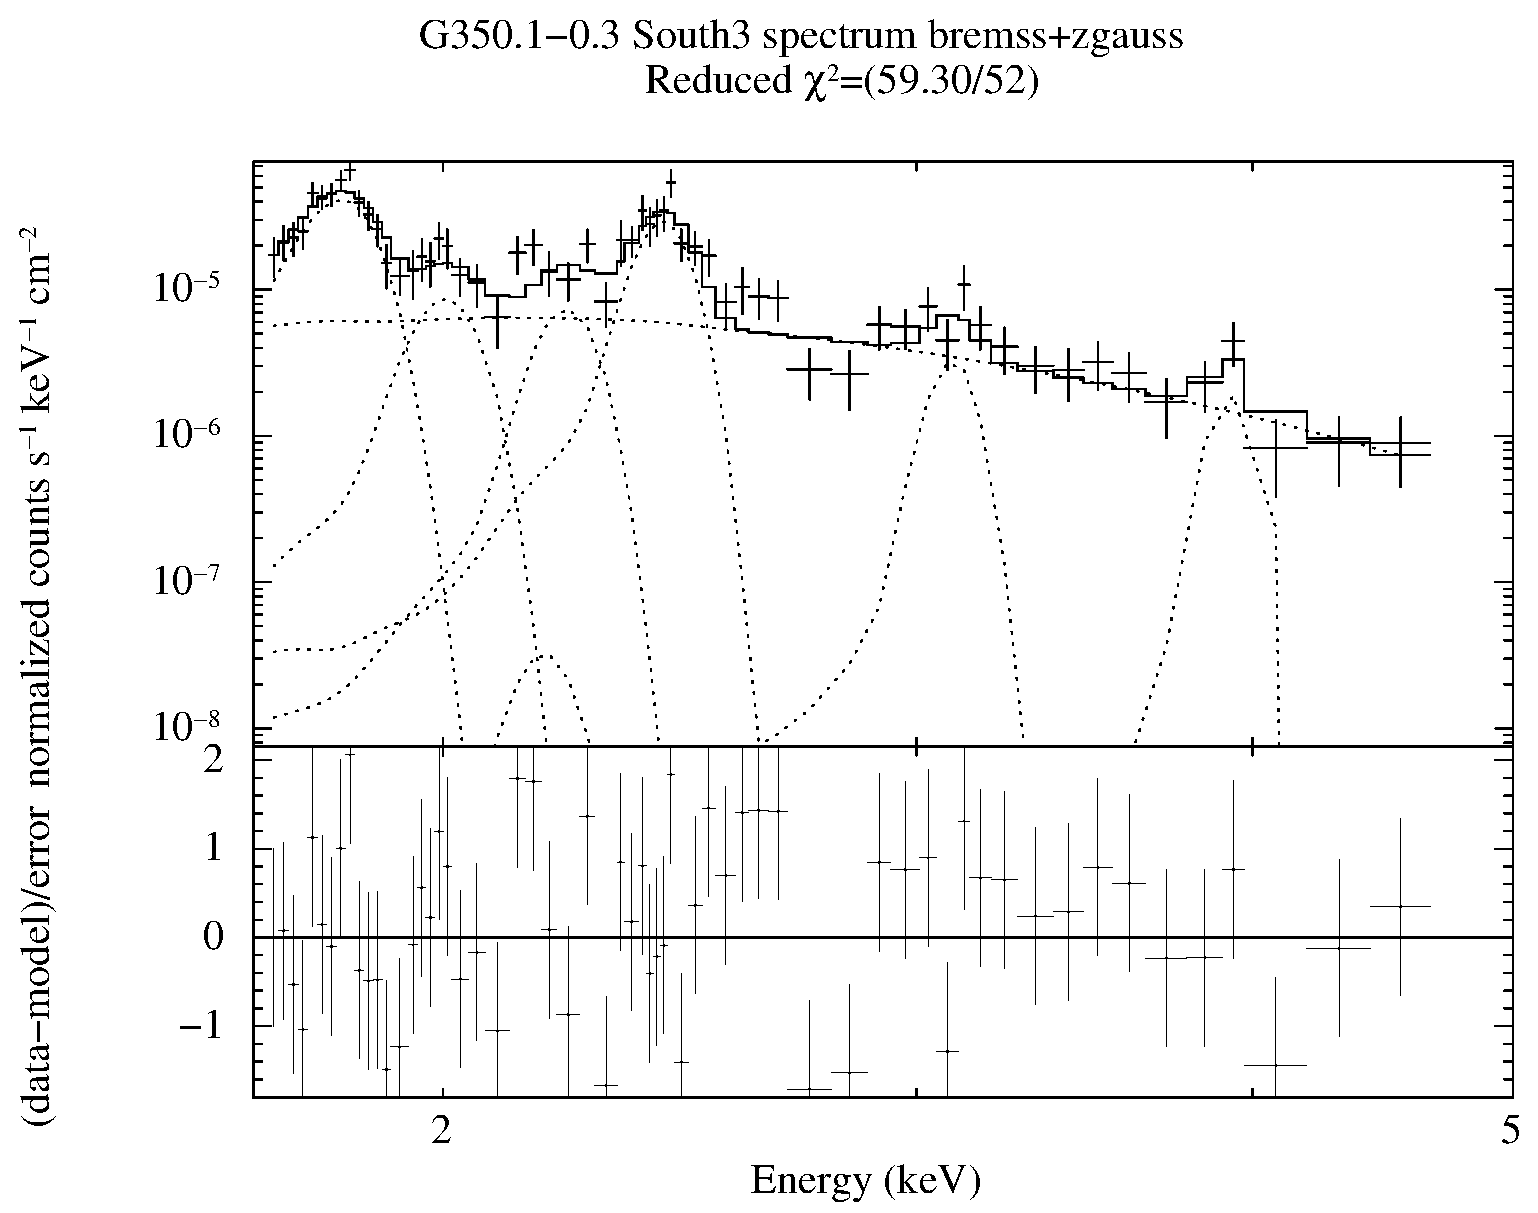
\includegraphics[scale=0.30]{./ps/South3_bremss+zgaussian.eps}
\end{center}
\end{minipage}
\end{tabular}
\caption{左図:South3領域をtbabs$\times$(bremss+gaussian)を用いてフィッティングを行なったスペクトルとモデルとの$\chi$の値、右図:South3領域をtbabs$\times$(bremss+zgaussian)を用いてフィッティングを行なったスペクトルとモデルとの$\chi$の値}
\label{fig:brem_South3}
\end{center}
\end{figure}

~~ドップラーシフトの他に、プラズマの状態に関しての情報を得るために$tbabs*(vnei)$または$tbabs*(apec+vnei)$を用いた解析も行なった。

\begin{figure}[H]
\begin{center}
\begin{tabular}{cc}
\begin{minipage}{0.5\hsize}
\begin{center}
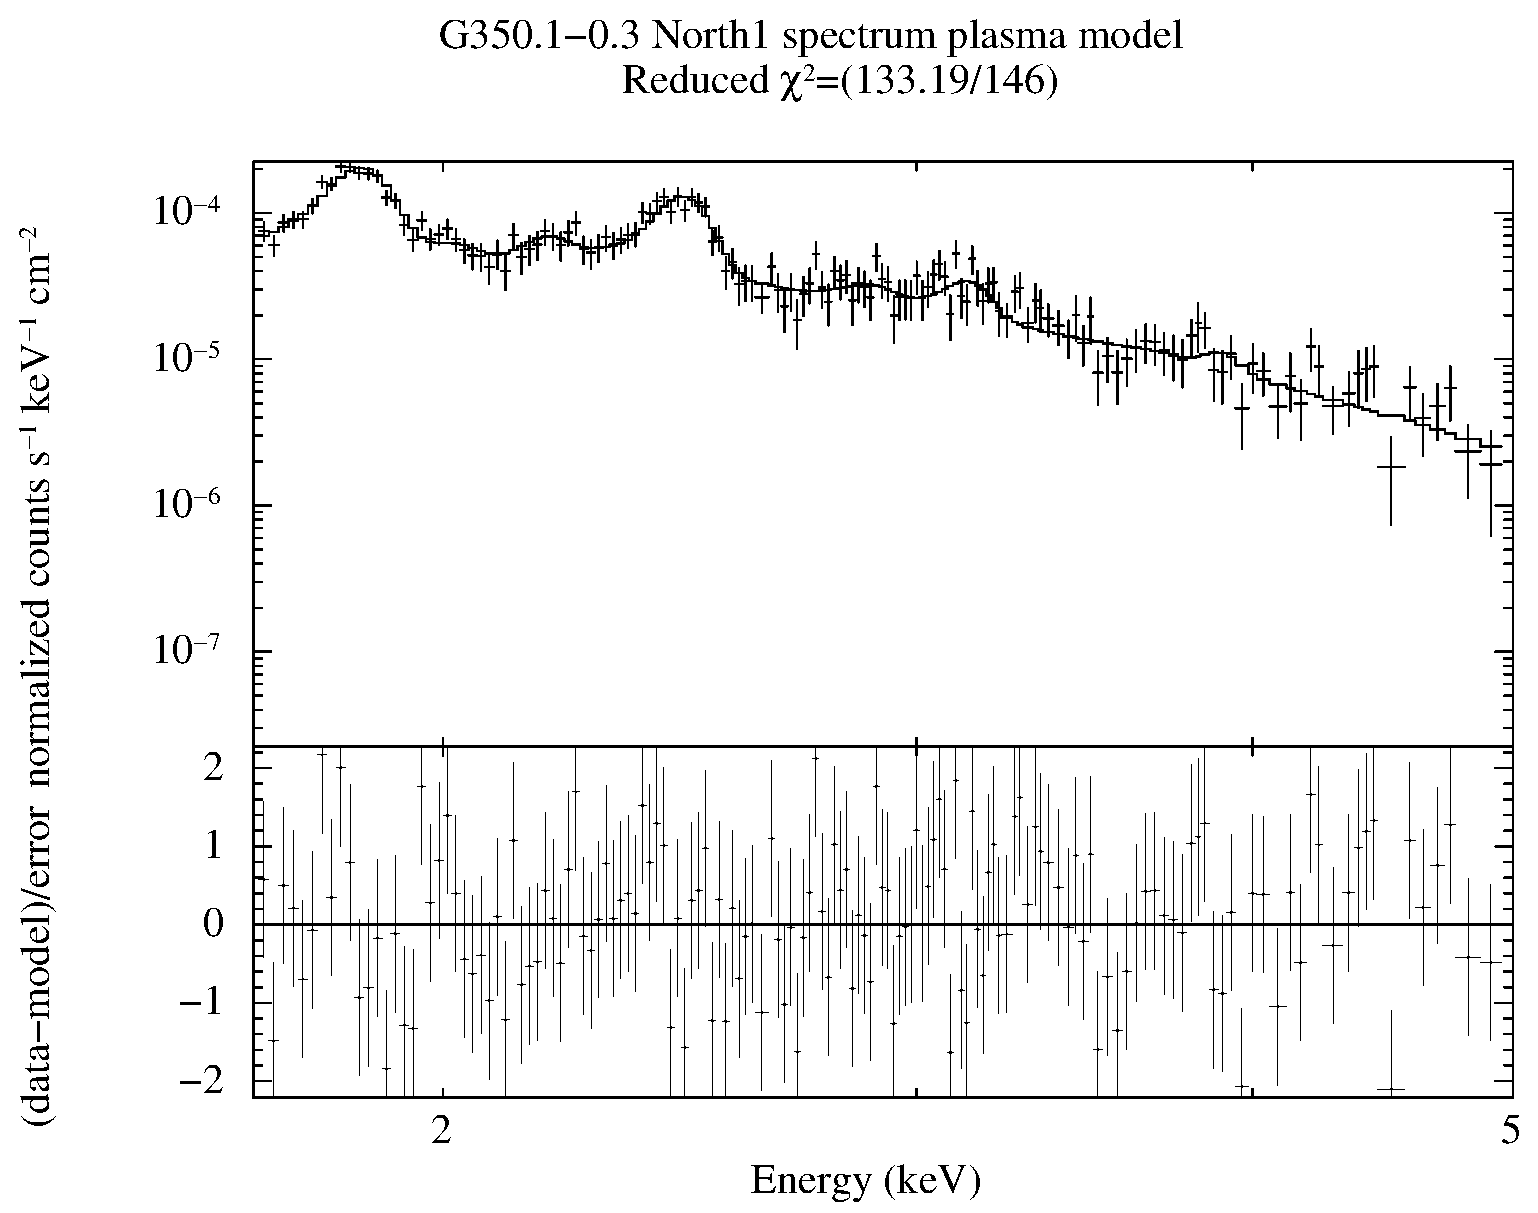
\includegraphics[scale=0.30]{./ps/North1_plasma.eps}
\end{center}
\end{minipage}
\begin{minipage}{0.5\hsize}
\begin{center}
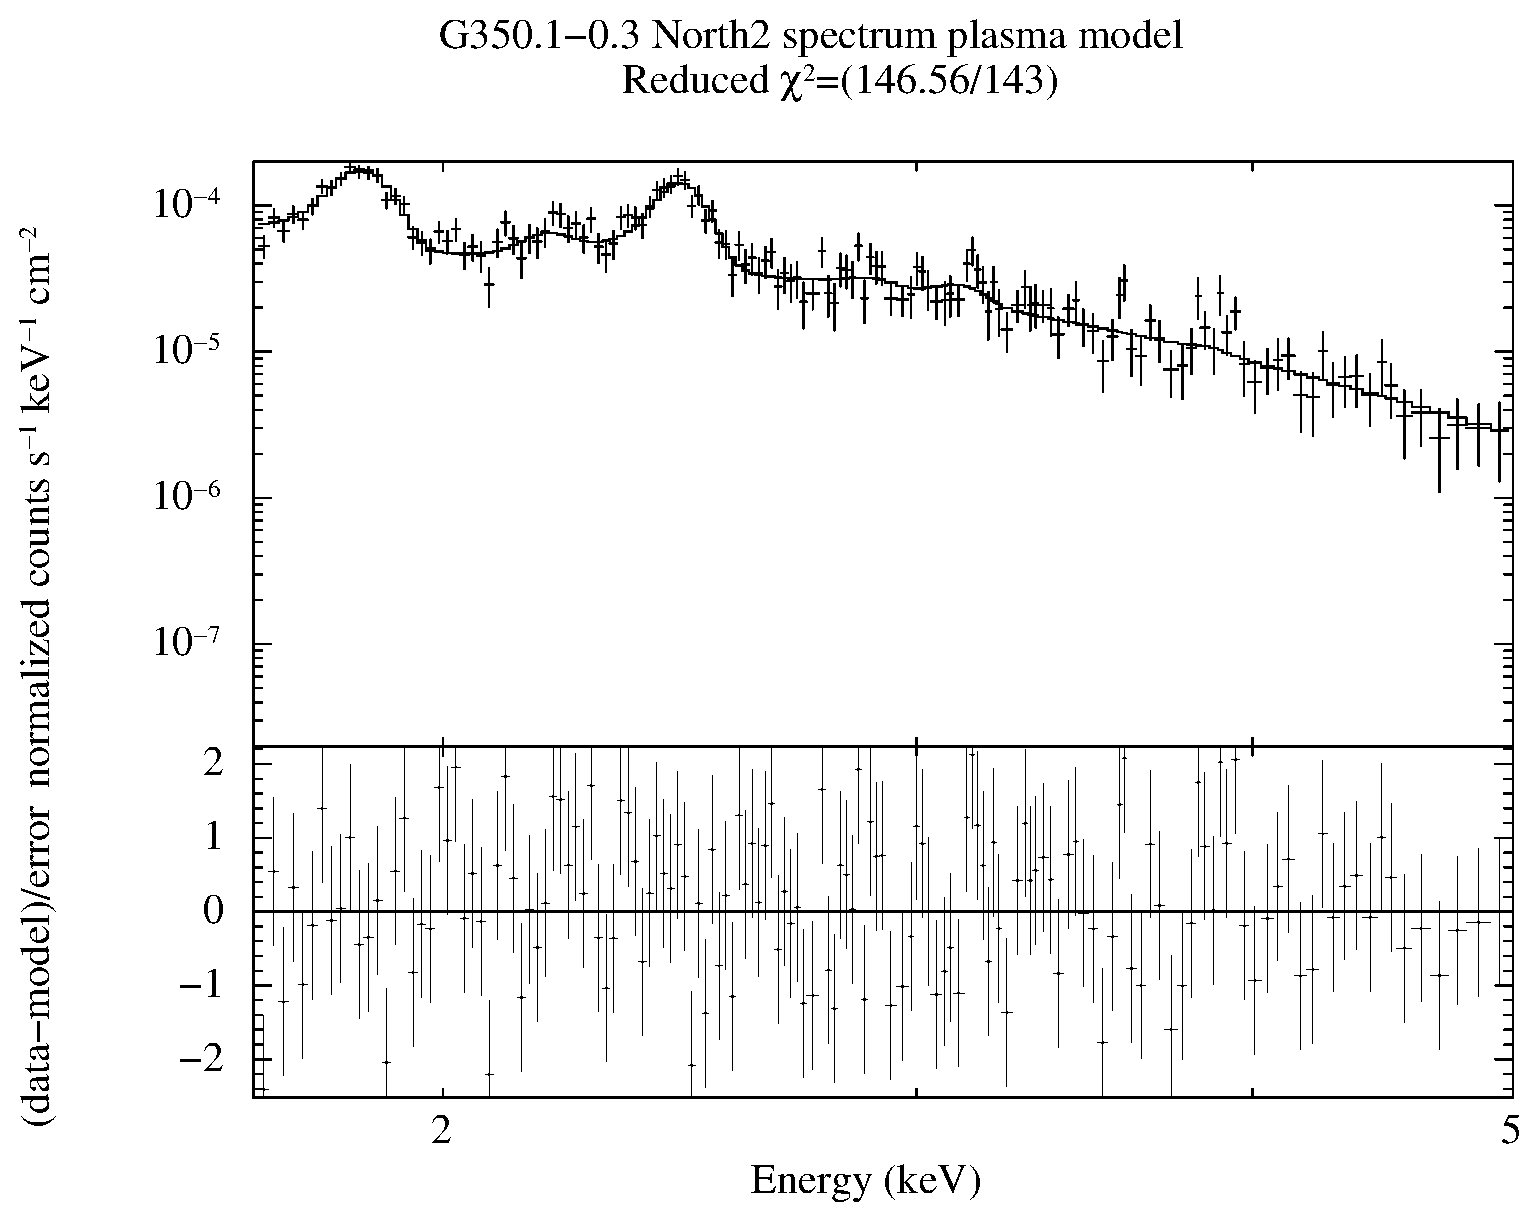
\includegraphics[scale=0.30]{./ps/North2_plasma.eps}
\end{center}
\end{minipage}
\end{tabular}
\caption{左図:North1領域をtbabs$\times$vneiを用いてフィッティングを行なったスペクトルとモデルとの$\chi$の値、右図:North2領域をtbabs$\times$vneiを用いてフィッティングを行なったスペクトルとモデルとの$\chi$の値}
\label{fig:plasma_North}
\end{center}
\end{figure}

\begin{figure}[H]
\begin{center}
\begin{tabular}{cc}
\begin{minipage}{0.5\hsize}
\begin{center}
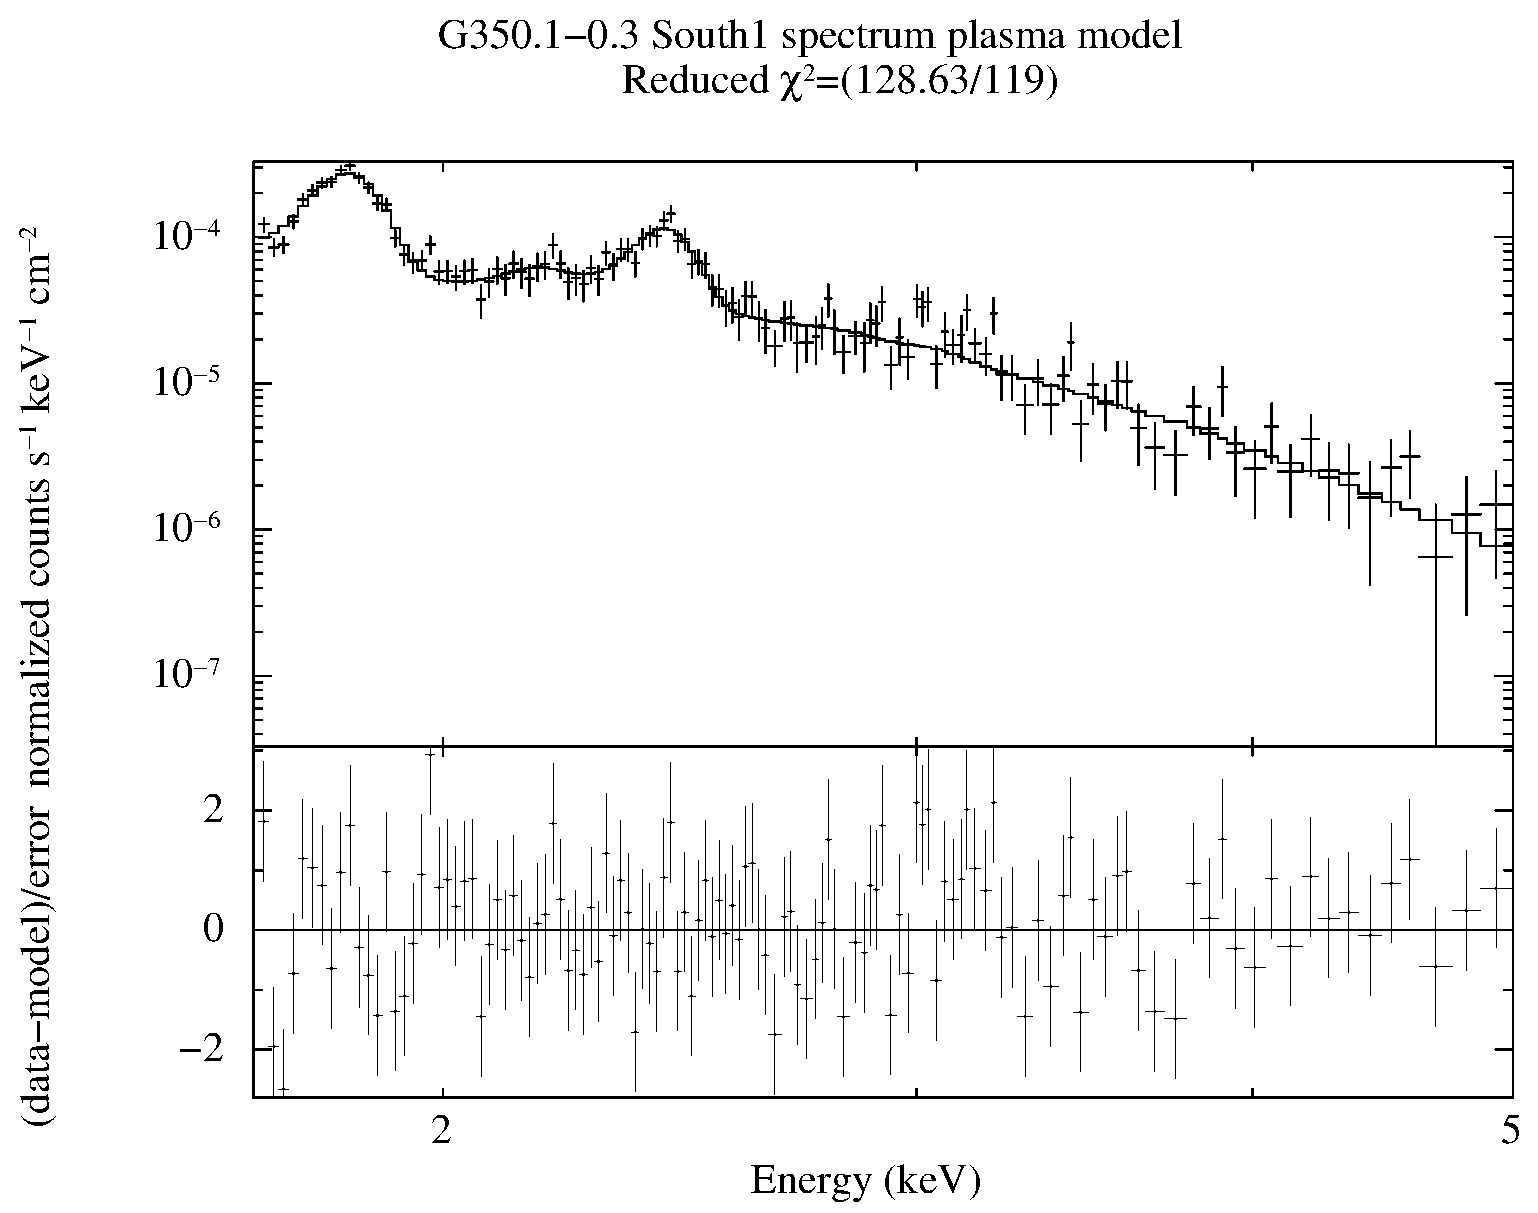
\includegraphics[scale=0.30]{./ps/South1_plasma.eps}
\end{center}
\end{minipage}
\begin{minipage}{0.5\hsize}
\begin{center}
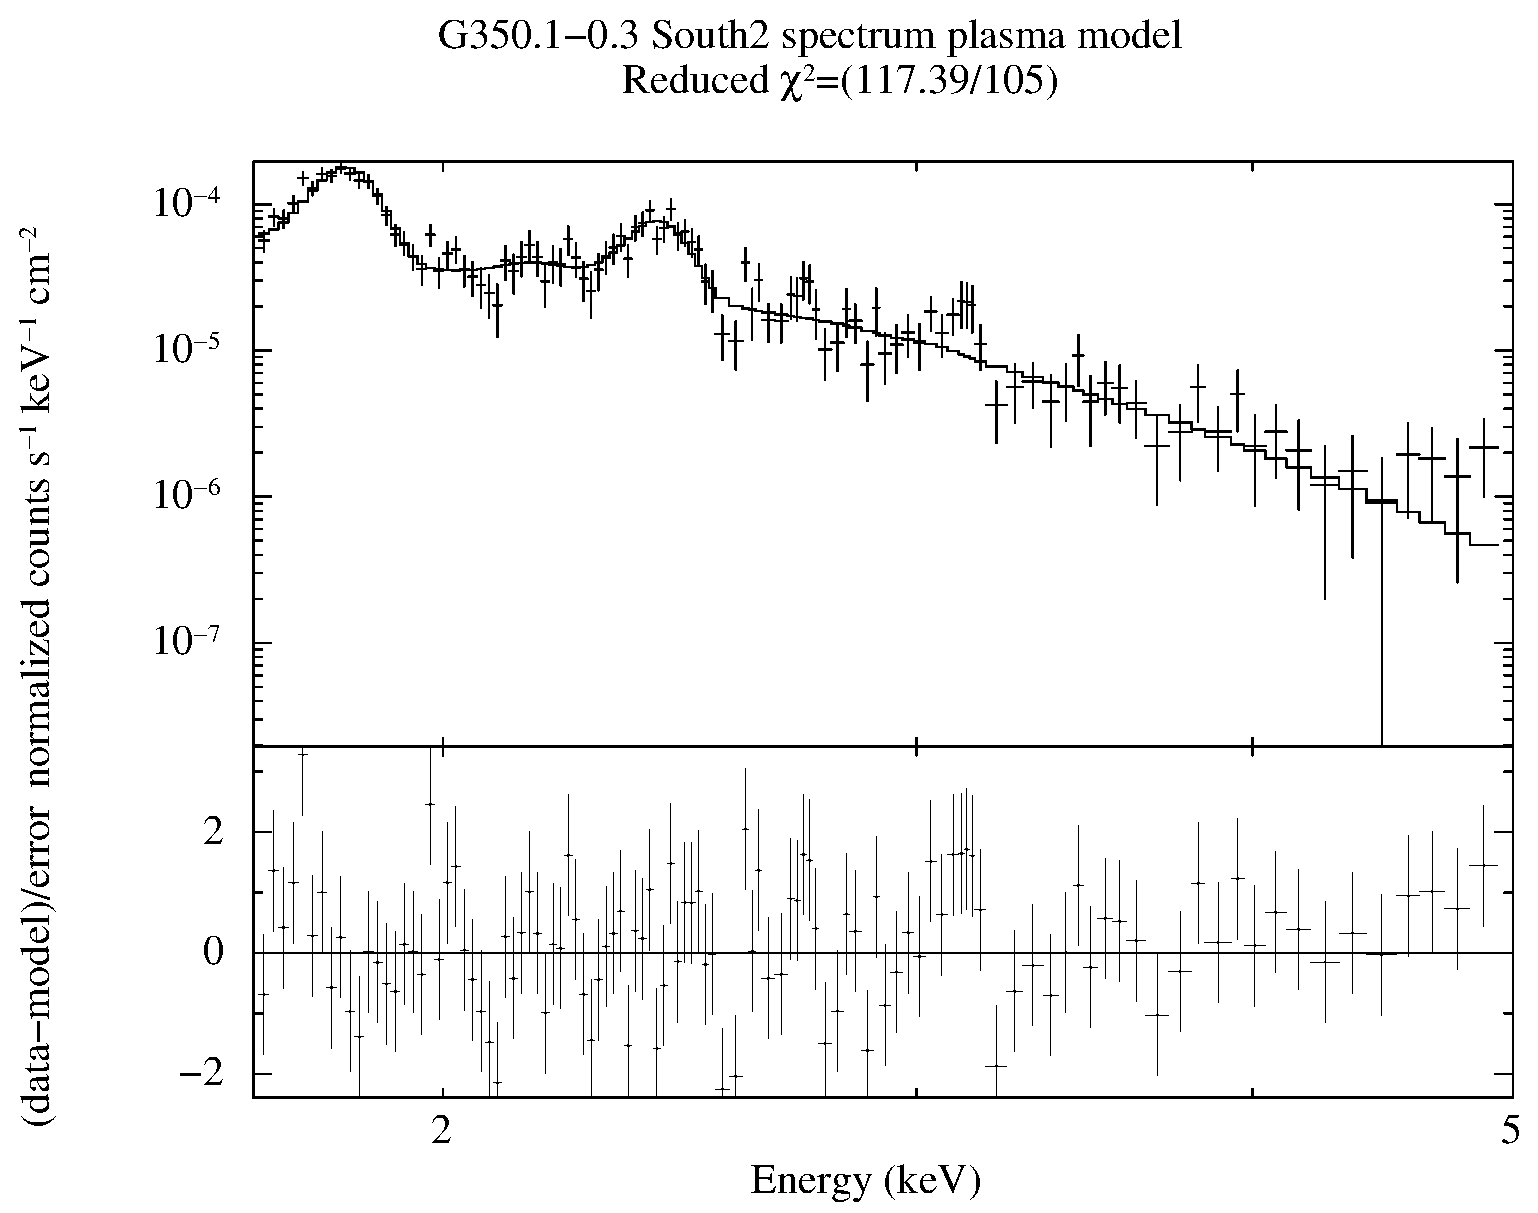
\includegraphics[scale=0.30]{./ps/South2_plasma.eps}
\end{center}
\end{minipage}
\end{tabular}
\caption{左図:South1領域をtbabs$\times$vneiを用いてフィッティングを行なったスペクトルとモデルとの$\chi$の値、右図:South2領域をtbabs$\times$vneiを用いてフィッティングを行なったスペクトルとモデルとの$\chi$の値}
\label{fig:plasma_South}
\end{center}
\end{figure}

\begin{figure}[H]
\begin{center}
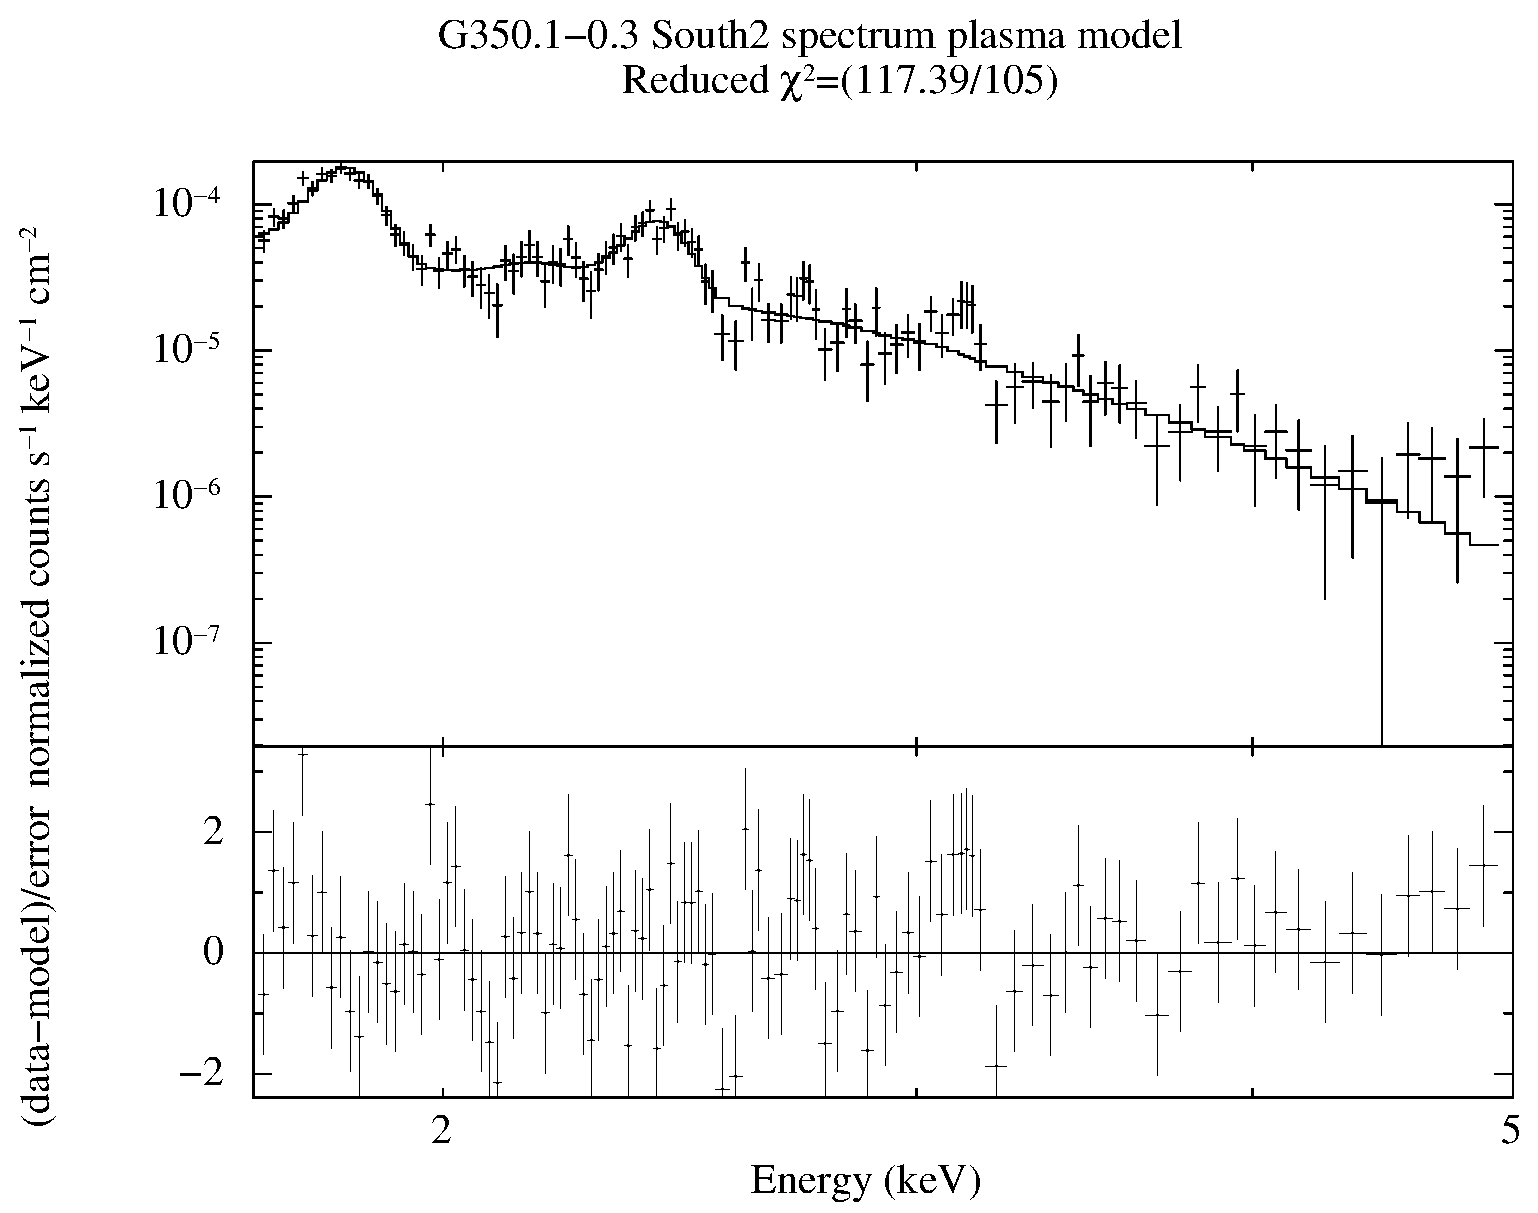
\includegraphics[scale=0.30]{./ps/South2_plasma.eps}
\caption{South3領域をtbabs$\times$vneiを用いてフィッティングを行なったスペクトルとモデルとの$\chi$の値}
\label{fig:plsma_South3}
\end{center}
\end{figure}


%%%-----------------------------%%%%%

\newpage
%------- Chandra analysis ------------
\section{議論}
\subsection{イジェクタの視線方向の速度}
スペクトル解析から求められたエネルギー中心値と以下の式\ref{eq:doppler-shift}を用いて、イジェクタの視線方向の速度を求めたところ、Fig.\ref{fig:velo}のようになった。
\begin{align}
  \frac{v}{c} = \frac{|E-E_{0}|}{E_{0}}
\label{eq:doppler-shift}
\end{align}

\begin{figure}[H]
\begin{center}
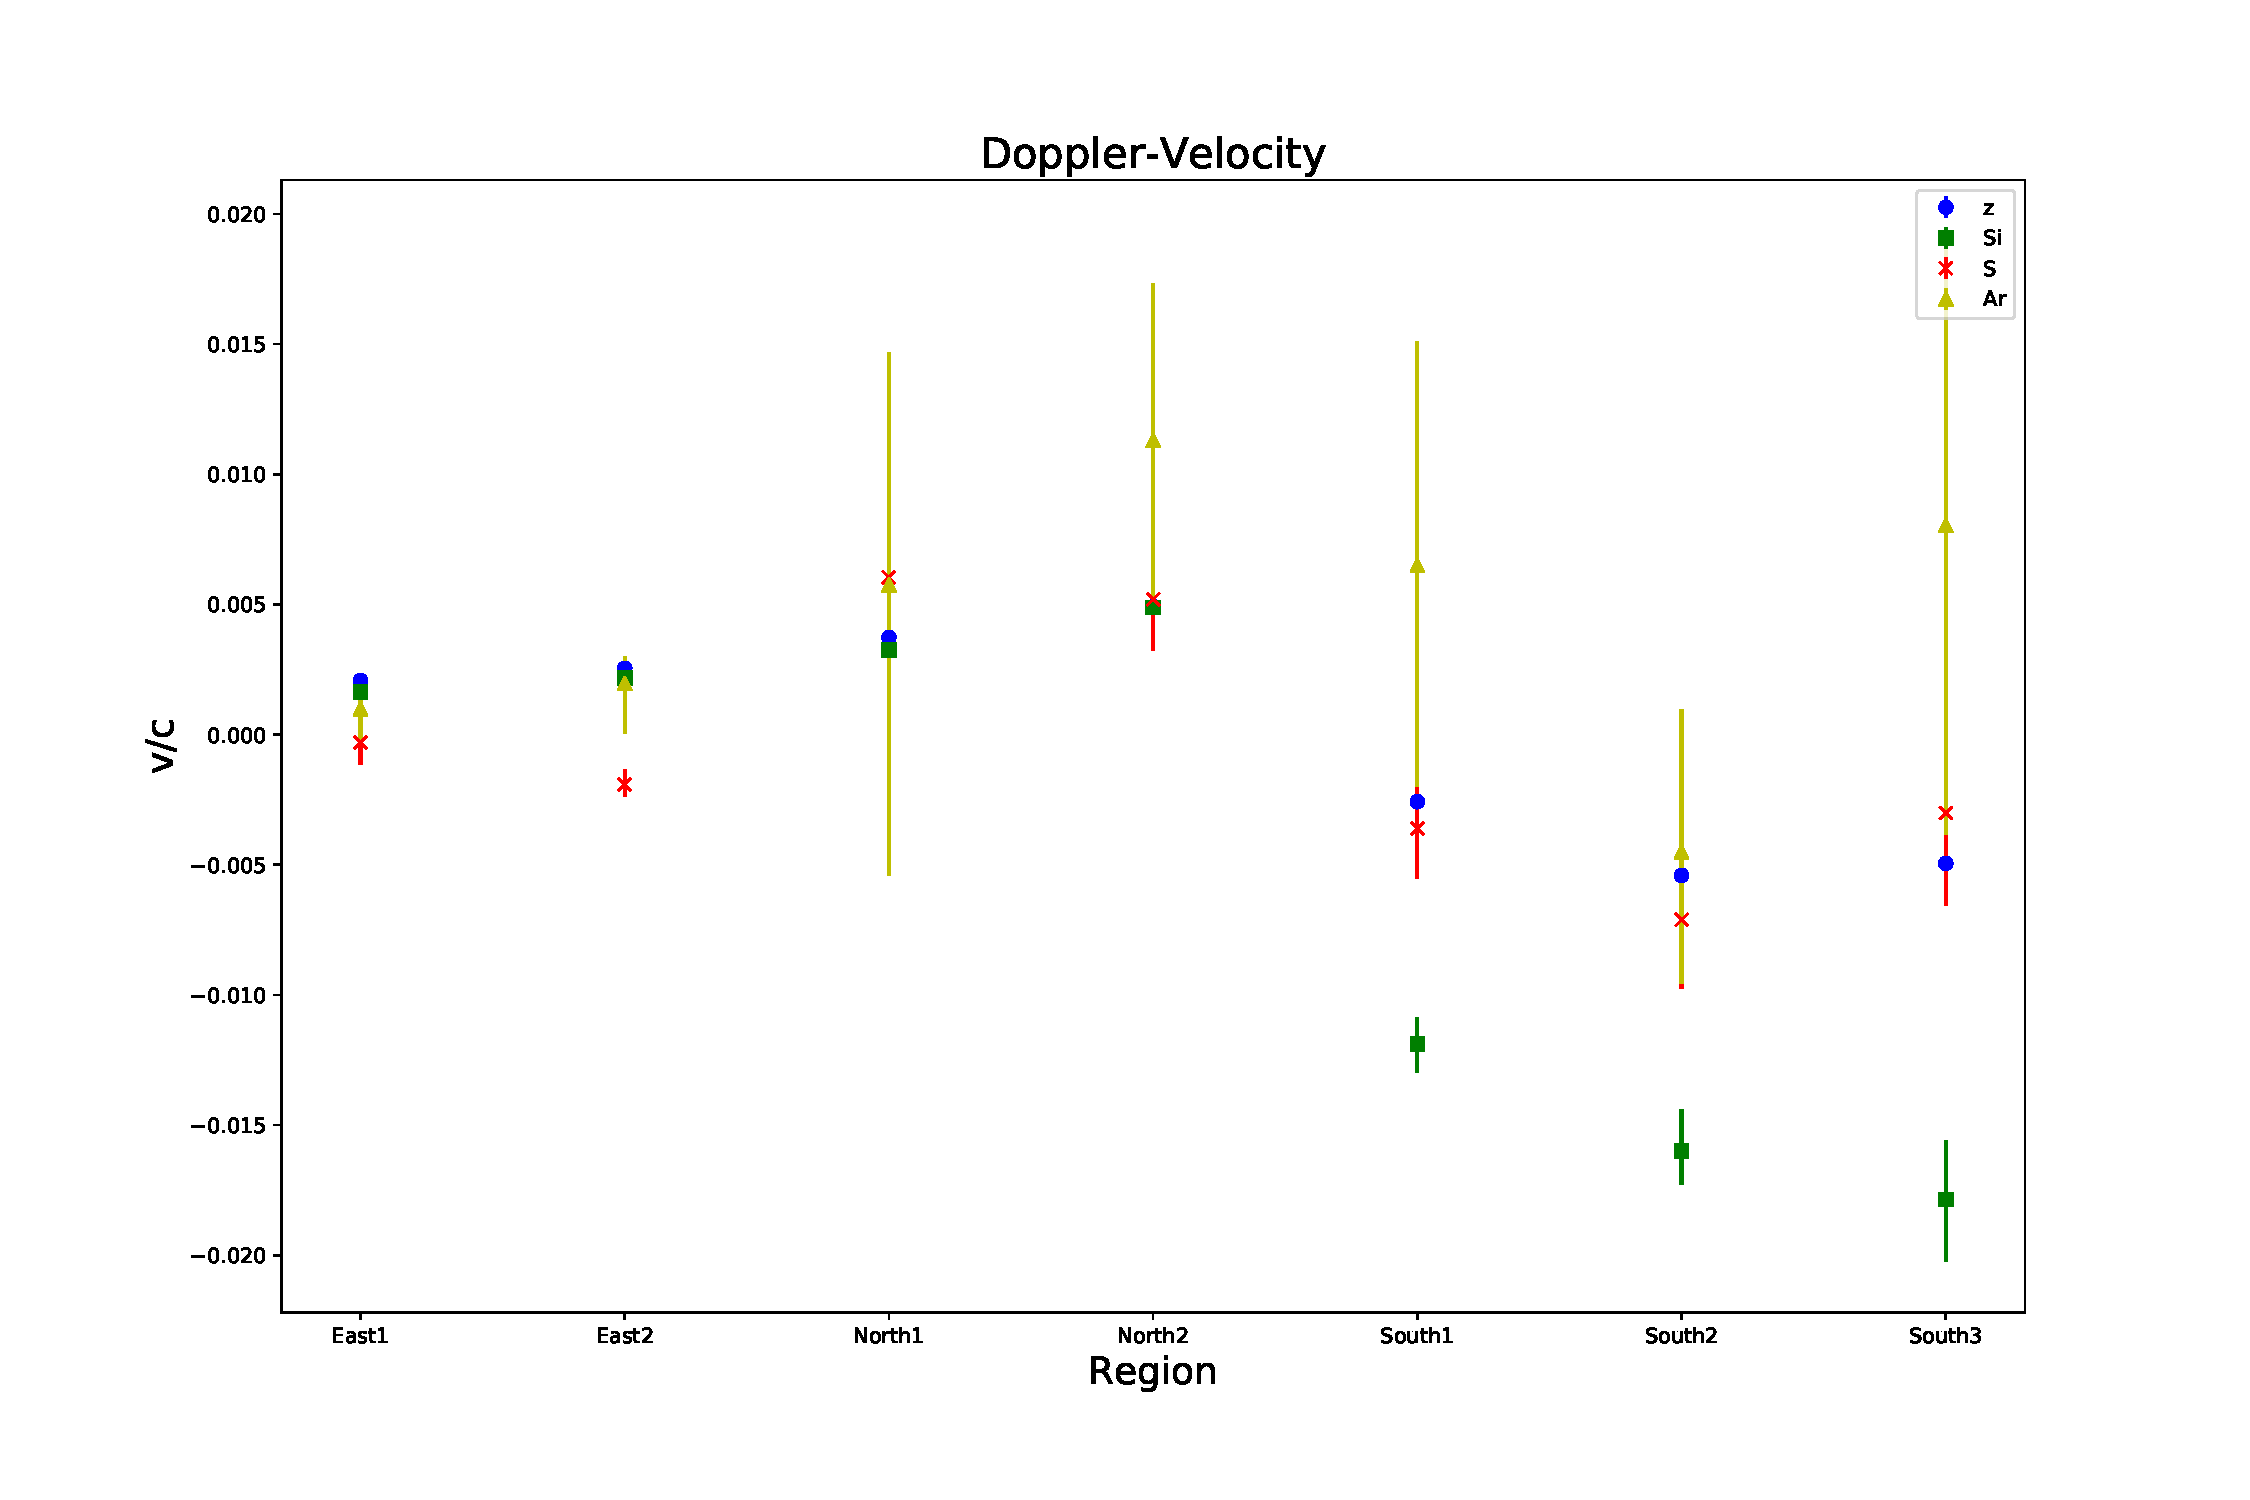
\includegraphics[scale=0.4]{./vel_lineofsight_1022.pdf}
\caption{ドップラー効果から求めた東側の放射領域に対する各元素の速度}
\label{fig:velo}
\end{center}
\end{figure}
Fig.\ref{fig:velo}から、このSNRの北側が観測者に対して近づく方向に、南側は遠ざかる方向に運動していることが示唆される。
この結果から、2pcの大きさをもつ巨大なプラズマ塊が北側と南側でそれぞれ視線方向に対して、$\rm{km/s}$、$\rm{km/s}$ではないかと考えられる。
  
\subsection{プラズマの年齢依存性}



\subsection{エネルギー中心値における温度・電離パラメーター依存性}
輝線のエネルギー中心がプラズマの元々の電子温度および電離パラメーターに依存している可能性があるため、Xspecのfakeitコマンドを用いて作成した温度と電離パラメーターがそれぞれ($n_e t =1e+9 \rm{s/cm^3}~kT=0.6 \rm{keV}$)、($n_e t =1e+10 \rm{s/cm^3}~kT=0.6 \rm{keV}$)、($n_e t =1e+9 \rm{s/cm^3}~kT=0.6 \rm{keV}$)でプラズマの$\rm{Si-He\alpha}$のエネルギー中心と観測値を比較してみる。その結果をFig.\ref{fig:centroid-simulation}に示す。合わせて、赤方偏移$\rm{z}$と$n_e t$、$kT$の関係、$n_e t$と$kT$の関係をFig.\ref{fig:plasma_corr}に示す。
\begin{figure}[H]
  \begin{center}
  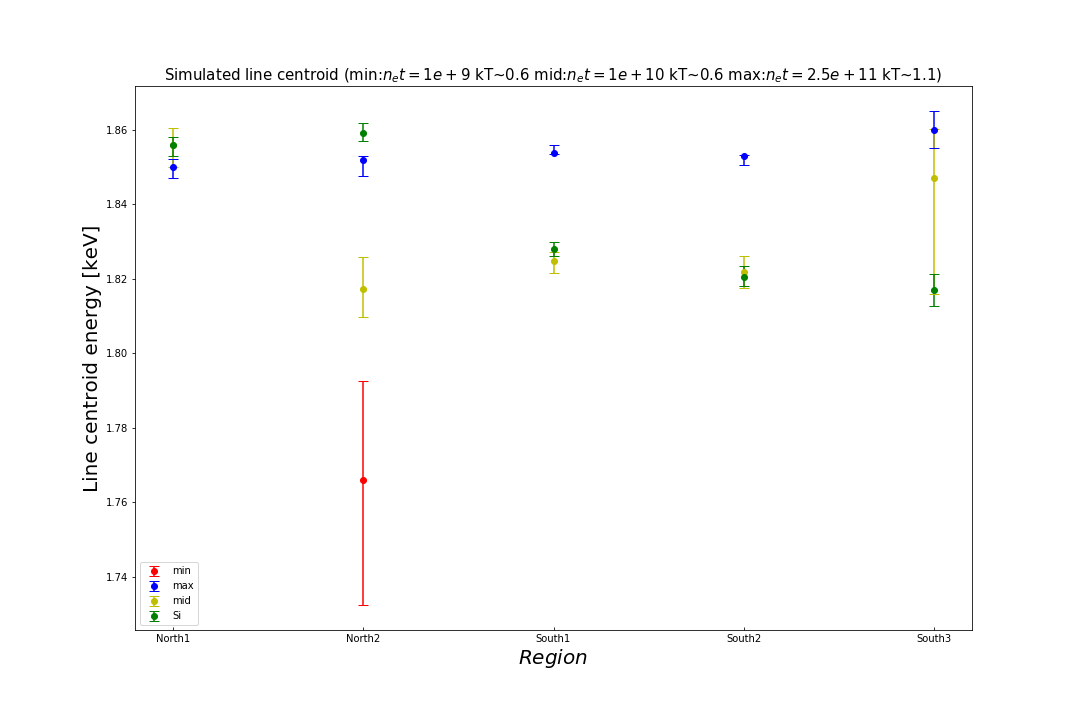
\includegraphics[scale=0.4]{./simulated_centroid_energy_vs_measured.png}
  \caption{観測値とシミュレーションスペクトルのエネルギー中心値の比較。シミュレーションスペクトルはそれぞれ$n_e t =1e+9 \rm{s/cm^3}~kT=0.6 \rm{keV}$、$n_e t =1e+10 \rm{s/cm^3}~kT=0.6 \rm{keV}$、$n_e t =1e+9 \rm{s/cm^3}~kT=0.6 \rm{keV}$}
  \label{fig:centroid-simulation}
  \end{center}
  \end{figure}

\begin{figure}[H]
\begin{center}
\begin{tabular}{ccc}
  
\begin{minipage}{0.5\hsize}
\begin{center}
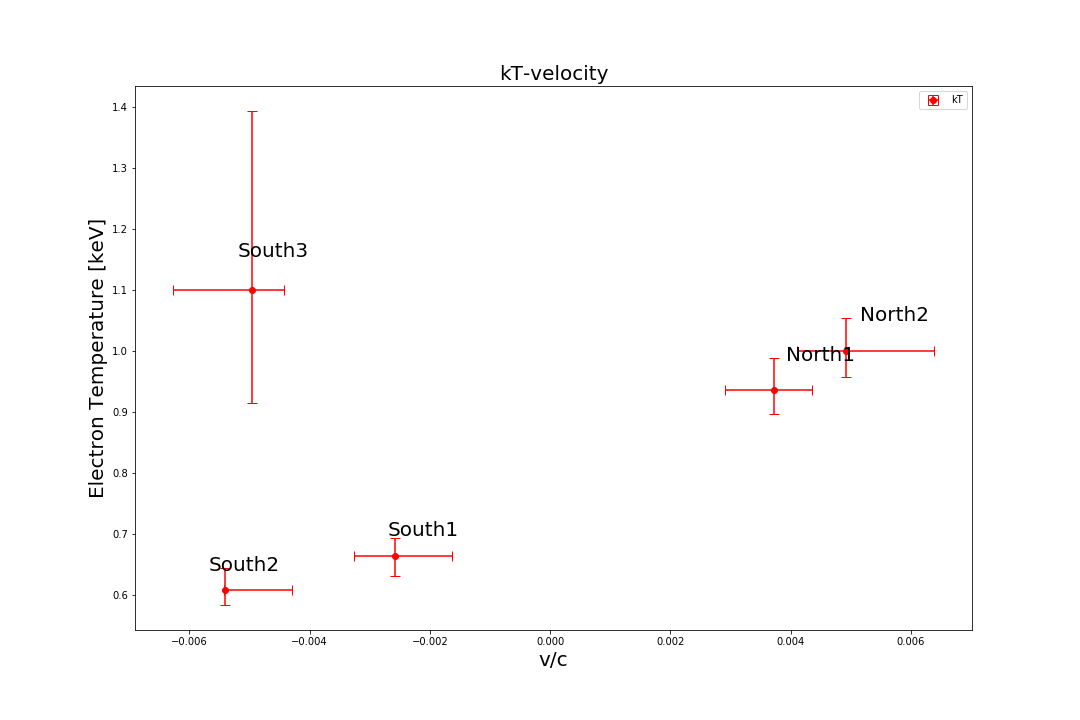
\includegraphics[scale=0.23]{./vel_vs_kT.png}
\end{center}
\end{minipage}

\begin{minipage}{0.5\hsize}
\begin{center}
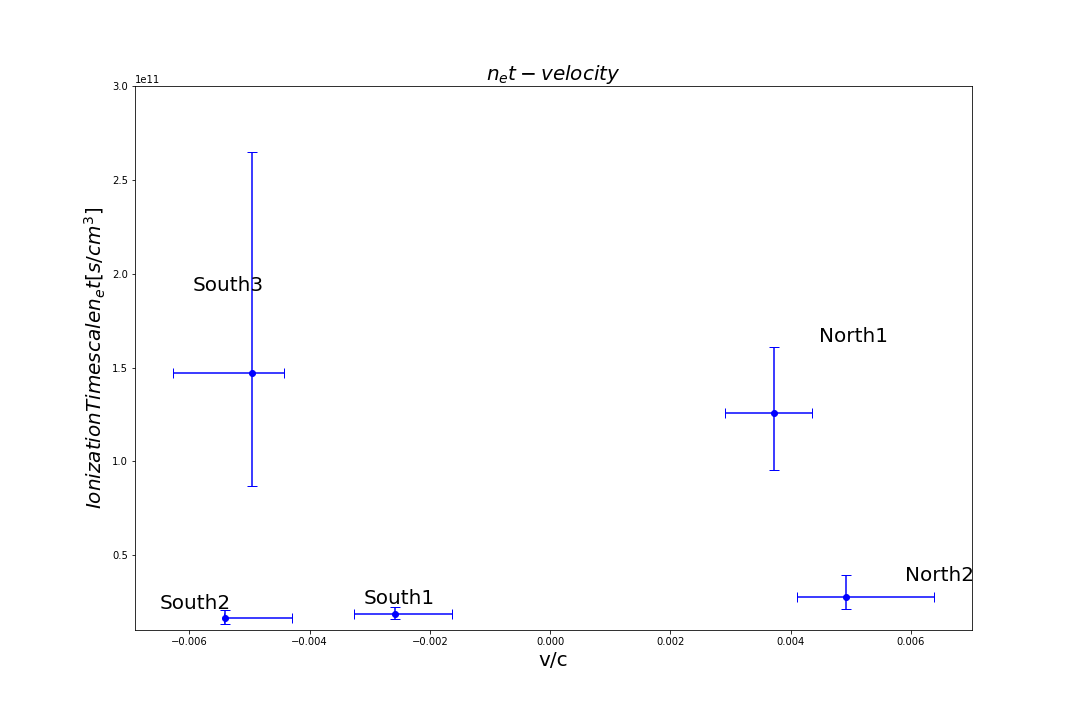
\includegraphics[scale=0.23]{./vel_vs_nt.png}
\end{center}
\end{minipage}
\end{tabular}
\caption{}
\label{fig:plasma_vel_corr}
\end{center}
\end{figure}

\begin{figure}[H]
\begin{center}
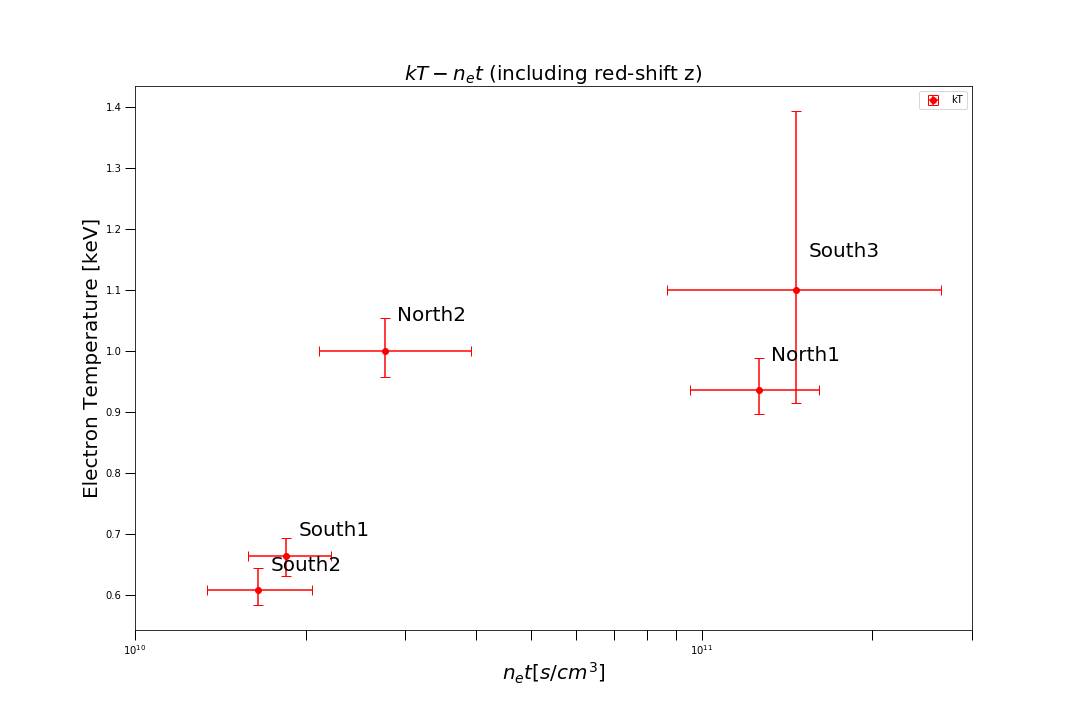
\includegraphics[scale=0.3]{./nt_vs_kT.png}
\label{fig:plasma_par_corr}
\end{center}
\end{figure}

これらの結果から、North2領域では、プラズマモデルから予想されるよりもエネルギー中心値が大きく、South2、South3領域では小さい値を取っていることがわかる。さらに、North1ではmaxとmidでエネルギー中心値がほとんど同じ値を取っていることから、North1では、ある程度の電離度以上でエネルギー中心値に変化がないことも考えられる。よって、North1もドップラーシフトを捕らえられているのではないかと考えることができる。South3は、実際にプラズマが取っている電子温度・電離パラメーターは今回のシミュレーションにしようした値よりも大きいので、このプラズマから観測されるエネルギー中心値はFig.\ref{fig:centroid-simulation}よりも大きくなることが予想される。このことから、これらの領域ではイジェクタが視線方向に運動していることが強く示唆される。

\subsection{輝線のエネルギー中心値シフトのシナリオの検証}


\subsection{非球対称超新星爆発モデルとの比較}

%%%%% 今回のChandraの観測データの解析によって、超新星残骸G350.1-0.3において、南側と北側の領域がそれぞれ視線方向に対して、遠ざかる向きと近づく向きに運動していることがわかった。
% この結果から、赤方偏移$\it{z}$を用いて視線方向の速度を求めると、南と北はそれぞれ、$v_{\rm{South}} \sim 1640^{+150}_{-130}$~km/s、$v_{\rm{North}} \sim 1570^{+330}_{-240}$~km/sであるとわかる。さらに、天体までの距離$\it{d}$を$d \sim 4.5~\rm{kpc}$\cite{Gaensler2008}と仮定すると、天体までの距離と楕円の長軸の大きさを用いて、南と北の領域の大きさはそれぞれ、$R_{South} \sim 0.95$~pc、$R_{North} \sim 1.14$~pcとなる。
% このことから、巨大なプラズマ塊が光速の$\sim \pm 0.5 \%$程度で運動していることがわかる。この結果から、この超新星残骸が極端に非対称な超新星爆発によって誕生したことが強く示唆される。\\
% 今後はESAのXMM-Newtonを用いた同様の解析によって、今回のChandraのデータを用いた解析による結果を確認することを予定している。この他、ドップラー効果の面から非対称性爆発が示唆されたことから、Chandraの空間分解能を活かし、より細かな領域に分割し、それぞれの領域でスペクトル解析することで、どのような超新星爆発モデルによってこの超新星爆発が再現できるのか既存の理論と照らし合わせて確かめていきたい。

\section{今後の展望}
\subsection{ひとみ代替機による観測シミュレーション}
\subsection{時間変動解析}

%%%%%%%%%%%%%%%%%%%%%%%%%%%%
%-------  Reference  -----------

\vspace{-1mm}
\setlength{\columnsep}{0.4pt}
%\setlength{\columnseprule}{0.4pt}
\setlength{\columnwidth}{10mm}
\begin{thebibliography}{5}
  \vspace{-5mm}
  \begin{multicols}{2}
    \vspace{-2mm}
		\bibitem{toshikisato}
		Toshiki Sato 博士論文 2018
    \label{toshikisato}

    \vspace{-2mm}
    \bibitem{Yasumi2014}
    Yasumi, M. et al. 2014, Pasj, 66, 68
    \label{Yasumi2014}

    \vspace{-2mm}
    \bibitem{2010ApJ...725..894H}
    Hayato, A. et al. 2010, Apj, 725, 894
    \label{2010ApJ...725..894H}

    \vspace{-2mm}
    \bibitem{Gaensler2008}
    Gaensler, B.~M. et al. 2008, ApjL, 680, L37
    \label{Gaensler2008}


  \end{multicols}

\end{thebibliography}



\end{document}
